\documentclass[12pt]{extreport}
\usepackage{subfigure}
\usepackage{fontspec}
\usepackage{polyglossia}
\setmainlanguage{vietnamese}
\usepackage[left=3.50cm, right=2.00cm, top=3.50cm, bottom=3.00cm]{geometry}
\usepackage{fancybox,graphicx}
\usepackage{mathrsfs}
\usepackage{amsfonts}
\usepackage{longtable,array}
\usepackage{multirow}
\newlength\mylength
\newcolumntype{C}[1]{>{\centering\arraybackslash}p{#1}}
\usepackage[intlimits]{amsmath}
\usepackage{array}
\usepackage[unicode]{hyperref}
\usepackage{algorithm}
\usepackage{algorithmicx}
\makeatletter
\renewcommand{\ALG@name}{Thuật toán}
\makeatother
\usepackage{algpseudocode}
\usepackage{amsxtra,amssymb,latexsym,amscd,amsthm}
\usepackage{enumitem}
\usepackage{tikz}
\usetikzlibrary{shapes.geometric}
\usetikzlibrary{positioning,automata}
\usepackage{scrextend}
\usepackage{longfbox}
\usepackage{float}
\usepackage{booktabs}

\newtheorem{pro}{Bài toán}
\newtheorem*{constr}{Ràng buộc}
\newtheorem*{calfunc}{Các hàm được thực thi}
\newtheorem*{Sol}{Giải thuật}
\newtheorem*{Anal}{Phân tích giải thuật}

\usepackage{fancyhdr}
\pagestyle{fancy}
\lhead{}
\chead{}
\rhead{Chuyên đề Công nghệ Phần mềm}
\lfoot{}
\cfoot{\thepage}
\rfoot{}

\usepackage{xcolor}
\usepackage{listings}

\definecolor{mGreen}{rgb}{0,0.6,0}
\definecolor{mGray}{rgb}{0.5,0.5,0.5}
\definecolor{mPurple}{rgb}{0.58,0,0.82}
\definecolor{backgroundColour}{rgb}{0.95,0.95,0.92}

\lstdefinestyle{CStyle}{
	backgroundcolor=\color{backgroundColour},
	commentstyle=\color{mGreen},
	keywordstyle=\color{magenta},
	numberstyle=\tiny\color{mGray},
	stringstyle=\color{mPurple},
	basicstyle=\footnotesize\ttfamily,
	breakatwhitespace=false,
	breaklines=true,
	captionpos=b,
	keepspaces=true,
	numbers=left,
	numbersep=5pt,
	showspaces=false,
	showstringspaces=false,
	showtabs=false,
	tabsize=2,
	language=C
}

\graphicspath{{./images/}}

\setlength{\parindent}{0pt}
\setlength{\parskip}{0.4\baselineskip}

\begin{document}

%=============================================================
% TITLE PAGE
%=============================================================
\thispagestyle{empty}
\thisfancypage{
	\setlength{\fboxsep}{0pt}
	\fbox}{}

\begin{center}
	{\fontsize{13pt}{1}\selectfont\textbf{HỌC VIỆN CÔNG NGHỆ BƯU CHÍNH VIỄN THÔNG}}
	\\
	{\fontsize{13pt}{1}\selectfont\textbf{KHOA CÔNG NGHỆ THÔNG TIN 1}}
	\\
	\textbf{--------------------  o0o  ---------------------}\\[1cm]
	
\includegraphics[width=0.35\textwidth]{img19.png} \\[1.2cm]
	\textbf{{\large BÁO CÁO CHUYÊN ĐỀ CÔNG NGHỆ PHẦN MỀM}}\\[1cm]
	\textbf{{\large CÁC THUẬT TOÁN ĐỐI SÁNH MẪU}}\\[0.2cm]
	\textbf{{\large (PATTERN MATCHING ALGORITHMS)}}\\[1cm]
\end{center}
\begin{flushleft}
	\hspace{2.7cm} \textbf{Họ và tên\hspace{2.74cm}:\hspace{0.2cm}Nguyễn Hoàng Tùng}\\[0.2cm]
	\hspace{2.7cm} \textbf{Mã sinh viên\hspace{2.07cm}:\hspace{0.2cm}B22DCDT294}\\[0.2cm]
	\hspace{2.7cm} \textbf{Lớp\hspace{4cm}:\hspace{0.2cm}E22CNPM03}\\[0.2cm]
	\hspace{2.7cm} \textbf{Hệ đào tạo\hspace{2.5cm}:\hspace{0.2cm}Chính quy}\\[0.2cm]
	\hspace{2.7cm} \textbf{Giảng viên hướng dẫn\hspace{0.2cm}:\hspace{0.2cm}TS. Nguyễn Duy Phương}\\[0.2cm]
\end{flushleft}

\vspace{1.0cm}
\begin{center}
	\textbf{{\large Hà Nội - 2026}}\\
\end{center}

%=============================================================
% TABLE OF CONTENTS
%=============================================================
\tableofcontents

%=============================================================
\chapter{Tổng quan}
%=============================================================

Các thuật toán tìm kiếm mẫu từ \textbf{trái sang phải} gồm:
\begin{itemize}
	\item Thuật toán Brute Force
	\item Search with an automaton
	\item Thuật toán Karp-Rabin
	\item Thuật toán Shift Or
	\item Thuật toán Morris-Pratt
	\item Thuật toán Knuth-Morris-Pratt
	\item Thuật toán Apostolico-Crochemore
	\item Thuật toán Not So Naïve
\end{itemize}

Các thuật toán tìm kiếm mẫu từ \textbf{phải sang trái} gồm:
\begin{itemize}
	\item Thuật toán Boyer-Moore
	\item Thuật toán Turbo-BM
	\item Thuật toán Quick Search
	\item Thuật toán Tuned-Boyer-Moore
	\item Thuật toán Zhu-Takaoka
	\item Thuật toán Berry-Ravindran
	\item Thuật toán Apostolico-Giancarlo
\end{itemize}

Các thuật toán tìm kiếm mẫu từ \textbf{vị trí xác định} gồm:
\begin{itemize}
	\item Thuật toán Colussi
	\item Thuật toán Skip Search
	\item Thuật toán Alpha Skip Search
\end{itemize}

Các thuật toán tìm kiếm mẫu từ \textbf{vị trí bất kỳ} gồm:
\begin{itemize}
	\item Thuật toán Horspool
	\item Thuật toán Smith
	\item Thuật toán Raita
\end{itemize}

%=============================================================
\chapter{Tìm kiếm mẫu từ trái sang phải}
%=============================================================

\section{Thuật toán Brute Force}

\subsection{Trình bày thuật toán}

Thuật toán Brute Force kiểm tra tất cả vị trí trong đoạn văn bản từ vị trí 0 đến $n - m$, xem liệu mẫu (pattern) có khớp ngay vị trí bắt đầu không. Sau mỗi lần kiểm tra, nó dịch mẫu sang phải 1 vị trí. Đặc điểm: không cần pha tiền xử lý, bộ nhớ cần dùng cố định.

\subsection{Đánh giá độ phức tạp thuật toán}

\begin{itemize}
	\item Độ phức tạp pha thực thi là $O(m \times n)$.
\end{itemize}

\subsection{Kiểm nghiệm thuật toán}

Giả sử ta có 2 mảng ký tự $y$ và $x$. Ta tiến hành tìm mảng $x$ trong mảng $y$ với:
\begin{itemize}
	\item $x = \texttt{GCAGAGAG}$, độ dài $m = 8$
	\item $y = \texttt{GCATCGCAGAGAGTATACAGTACG}$, độ dài $n = 24$
\end{itemize}

Pha tìm kiếm (các bước so sánh từ trái sang phải):

\begin{figure}[H]
	\centering
	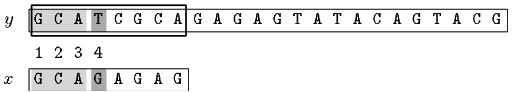
\includegraphics[width=0.9\textwidth]{img57.jpg}
	\caption{Lần 1: So sánh từ vị trí 0}
\end{figure}
\begin{figure}[H]
	\centering
	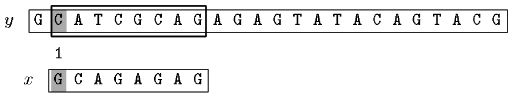
\includegraphics[width=0.9\textwidth]{img58.jpg}
	\caption{Lần 2}
\end{figure}
\begin{figure}[H]
	\centering
	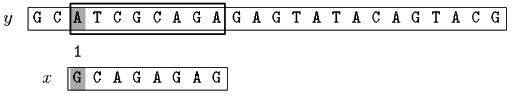
\includegraphics[width=0.9\textwidth]{img59.jpg}
	\caption{Lần 3}
\end{figure}
\begin{figure}[H]
	\centering
	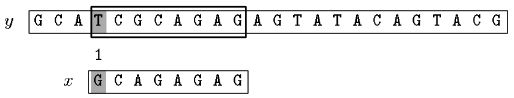
\includegraphics[width=0.9\textwidth]{img60.jpg}
	\caption{Lần 4}
\end{figure}
\begin{figure}[H]
	\centering
	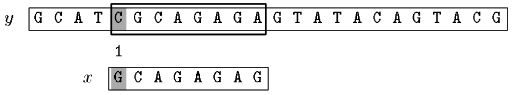
\includegraphics[width=0.9\textwidth]{img61.jpg}
	\caption{Lần 5}
\end{figure}
\begin{figure}[H]
	\centering
	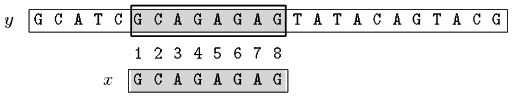
\includegraphics[width=0.9\textwidth]{img62.jpg}
	\caption{Lần 6: Tìm thấy $x$ tại vị trí 5}
\end{figure}
\begin{figure}[H]
	\centering
	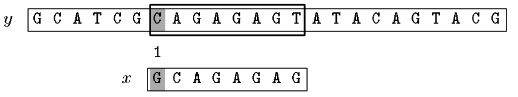
\includegraphics[width=0.9\textwidth]{img63.jpg}
	\caption{Lần 7}
\end{figure}
\begin{figure}[H]
	\centering
	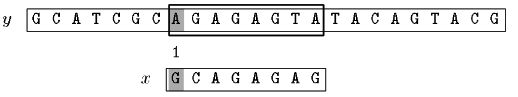
\includegraphics[width=0.9\textwidth]{img66.jpg}
	\caption{Lần 8}
\end{figure}
\begin{figure}[H]
	\centering
	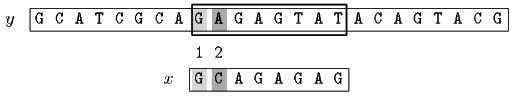
\includegraphics[width=0.9\textwidth]{img67.jpg}
	\caption{Lần 9}
\end{figure}
\begin{figure}[H]
	\centering
	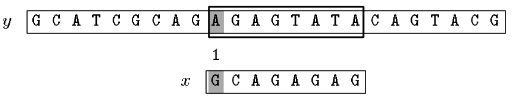
\includegraphics[width=0.9\textwidth]{img68.jpg}
	\caption{Lần 10}
\end{figure}
\begin{figure}[H]
	\centering
	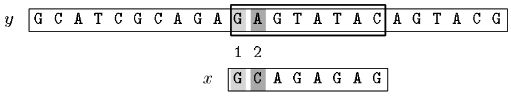
\includegraphics[width=0.9\textwidth]{img69.jpg}
	\caption{Lần 11}
\end{figure}
\begin{figure}[H]
	\centering
	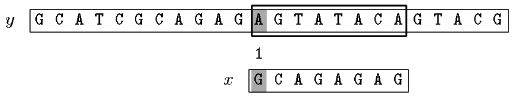
\includegraphics[width=0.9\textwidth]{img70.jpg}
	\caption{Lần 12}
\end{figure}
\begin{figure}[H]
	\centering
	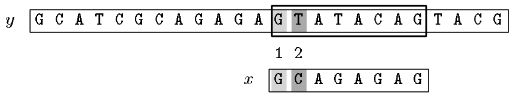
\includegraphics[width=0.9\textwidth]{img71.jpg}
	\caption{Lần 13}
\end{figure}
\begin{figure}[H]
	\centering
	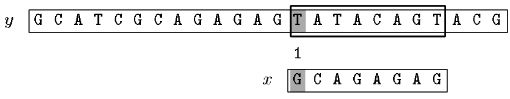
\includegraphics[width=0.9\textwidth]{img72.jpg}
	\caption{Lần 14}
\end{figure}
\begin{figure}[H]
	\centering
	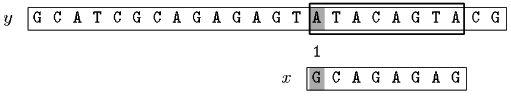
\includegraphics[width=0.9\textwidth]{img91.jpg}
	\caption{Lần 15}
\end{figure}
\begin{figure}[H]
	\centering
	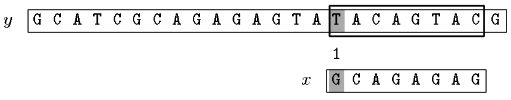
\includegraphics[width=0.9\textwidth]{img92.jpg}
	\caption{Lần 16}
\end{figure}
\begin{figure}[H]
	\centering
	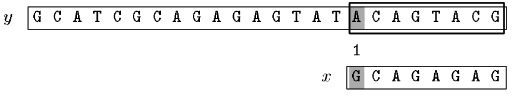
\includegraphics[width=0.9\textwidth]{img93.jpg}
	\caption{Lần 17: Kết thúc}
\end{figure}

Vậy ta thấy chỉ có lần 6 là tìm thấy mảng $x$ trong mảng $y$. Trong ví dụ trên, thuật toán Brute Force phải thực hiện 30 lần so sánh.

\subsection{Lập trình theo thuật toán}

\begin{lstlisting}[style=CStyle]
void BF(char *x, int m, char *y, int n) {
    int i, j;
    for (j = 0; j <= n - m; ++j) {
        for (i = 0; i < m && x[i] == y[i + j]; ++i);
        if (i >= m)
            printf("%d\n", j);
    }
}
\end{lstlisting}

%-----------------------------------------------------------
\section{Search with an automaton}
%-----------------------------------------------------------

\subsection{Trình bày thuật toán}

Thuật toán này xây dựng DFA (Deterministic Finite Automaton -- máy trạng thái hữu hạn xác định) giúp tìm kiếm mẫu trên văn bản một cách nhanh chóng.

\textbf{Định nghĩa máy trạng thái hữu hạn DFA:}

DFA là một bộ gồm $(Q, \Sigma, \delta: Q \times \Sigma \rightarrow Q, q_0 \in Q, F \subseteq Q)$. Trong đó:
\begin{itemize}
	\item $Q$ -- tập tất cả các tiền tố của mẫu $x = x_0 \ldots x_{m-1}$: $Q = \{\epsilon, x_0, x_0 x_1, \ldots, x_0 x_1 \ldots x_{m-1}\}$
	\item $q_0 = \epsilon$ -- trạng thái biểu diễn tiền tố rỗng.
	\item $F = x$ -- trạng thái biểu diễn tiền tố trùng với mẫu $x$.
	\item $\Sigma$ là tập các ký tự có trong mẫu $x$ và văn bản $y$.
	\item $\delta$ -- hàm chuyển tiếp: với mỗi $q \in Q$ và $c \in \Sigma$ thì $\delta(q, c) = qc$ khi $qc \in Q$; ngược lại $\delta(q, c) = p$ là hậu tố dài nhất của $qc$ mà cũng là tiền tố của $x$.
\end{itemize}

Trong thuật toán này, quá trình tìm kiếm được đưa về một quá trình biến đổi trạng thái automat. Mỗi trạng thái của automat sẽ đại diện cho số ký tự đang khớp của mẫu với văn bản. Khi đạt được trạng thái cuối cùng $F$ có nghĩa là đã tìm được một vị trí xuất hiện của mẫu.

\subsection{Đánh giá độ phức tạp thuật toán}

\begin{itemize}
	\item Pha tiền xử lý có độ phức tạp là $O(m \times \sigma)$.
	\item Pha tìm kiếm có độ phức tạp là $O(n)$ nếu DFA được chứa trong bảng truy cập trực tiếp, ngược lại $O(n \times \log \sigma)$.
\end{itemize}

\subsection{Kiểm nghiệm thuật toán}

Giả sử ta tìm kiếm mẫu $x = \texttt{abaa}$ trong văn bản $y = \texttt{ababbaabaaab}$.

Pha tiền xử lý -- tính DFA:
\[
\Sigma = \{a, b\};\quad Q = \{\epsilon, a, ab, aba, abaa\};\quad q_0 = \epsilon;\quad F = abaa
\]

Hàm chuyển tiếp $\delta(q, c)$:

\begin{center}
\begin{tabular}{|c|c|c|c|c|c|}
\hline
 & $\epsilon$ & $a$ & $ab$ & $aba$ & $\textcolor{red}{abaa}$ \\
\hline
$a$ & $a$ & $a$ & $aba$ & $\textcolor{red}{abaa}$ & $a$ \\
\hline
$b$ & $\epsilon$ & $ab$ & $\epsilon$ & $ab$ & $ab$ \\
\hline
\end{tabular}
\end{center}

\begin{figure}[H]
	\centering
	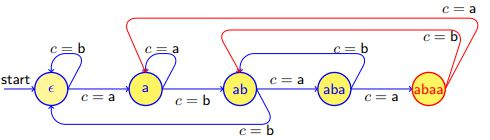
\includegraphics[width=0.9\textwidth]{img102.jpg}
	\caption{Sơ đồ DFA cho mẫu $x = \texttt{abaa}$}
\end{figure}

\[
q_{\text{next}} = \delta(q_{\text{curr}},\, c) =
\]
\begin{center}
\begin{tabular}{r|cc}
$q_{\text{curr}} \setminus c$ & \texttt{a} & \texttt{b} \\
\hline
$\epsilon$ & $a$ & $\epsilon$ \\
$a$ & $a$ & $ab$ \\
$ab$ & $aba$ & $\epsilon$ \\
$aba$ & \textcolor{red}{$abaa$} & $ab$ \\
\textcolor{red}{$abaa$} & $a$ & $ab$ \\
\end{tabular}
\end{center}

Pha tìm kiếm:

\begin{center}
\begin{tabular}{c | l | l@{\;}c@{\;}l}
\toprule
\textsc{Bước} & \textsc{Văn bản} & \multicolumn{3}{c}{\textsc{Trạng thái}} \\
\midrule
1  & \texttt{\textcolor{blue}{\underline{a}}babbaabaaab}                              & $\epsilon$ & $\rightarrow$ & $a$    \\
2  & \texttt{\textcolor{blue}{\underline{ab}}abbaabaaab}                              & $a$        & $\rightarrow$ & $ab$   \\
3  & \texttt{\textcolor{blue}{\underline{aba}}bbaabaaab}                              & $ab$       & $\rightarrow$ & $aba$  \\
4  & \texttt{ab\textcolor{blue}{\underline{ab}}baabaaab}                              & $aba$      & $\rightarrow$ & $ab$   \\
5  & \texttt{ababbaabaaab}                                                             & $ab$       & $\rightarrow$ & $\epsilon$ \\
6  & \texttt{ababb\textcolor{blue}{\underline{a}}abaaab}                              & $\epsilon$ & $\rightarrow$ & $a$    \\
7  & \texttt{ababba\textcolor{blue}{\underline{a}}baaab}                              & $a$        & $\rightarrow$ & $a$    \\
8  & \texttt{ababba\textcolor{blue}{\underline{ab}}aaab}                              & $a$        & $\rightarrow$ & $ab$   \\
9  & \texttt{ababba\textcolor{blue}{\underline{aba}}aab}                              & $ab$       & $\rightarrow$ & $aba$  \\
10 & \texttt{ababba\textcolor{red}{\underline{abaa}}ab}                               & $aba$      & $\rightarrow$ & \textcolor{red}{$abaa$} \\
11 & \texttt{ababba\textcolor{red}{abaa}\textcolor{blue}{\underline{a}}b}             & \textcolor{red}{$abaa$} & $\rightarrow$ & $a$ \\
12 & \texttt{ababbaabaa\textcolor{blue}{\underline{ab}}}                              & $a$        & $\rightarrow$ & $ab$   \\
\bottomrule
\end{tabular}
\end{center}

Tại bước thứ 11, thuật toán đã tìm thấy mẫu $x$ trong văn bản $y$.

\subsection{Lập trình theo thuật toán}

\begin{lstlisting}[style=CStyle]
#define MAX 256

int getNextState(char *pat, int m, int state, int x) {
    int ns, i;
    if (state < m && x == pat[state])
        return state + 1;
    for (ns = state; ns > 0; ns--) {
        if (pat[ns - 1] == x) {
            for (i = 0; i < ns - 1; i++)
                if (pat[i] != pat[state - ns + 1 + i])
                    break;
            if (i == ns - 1)
                return ns;
        }
    }
    return 0;
}

void computeTF(char *pat, int m, int TF[][MAX]) {
    int state, x;
    for (state = 0; state <= m; state++)
        for (x = 0; x < MAX; x++)
            TF[state][x] = getNextState(pat, m, state, x);
}

void finite_automata(char *pat, char *txt) {
    int i, state = 0;
    int m = strlen(pat), n = strlen(txt);
    int TF[m + 1][MAX];
    computeTF(pat, m, TF);
    for (i = 0; i <= n; i++) {
        state = TF[state][(unsigned char)txt[i]];
        if (state >= m)
            printf("Position: %d\n", i - m + 1);
    }
}
\end{lstlisting}

%-----------------------------------------------------------
\section{Thuật toán Karp-Rabin}
%-----------------------------------------------------------

\subsection{Trình bày thuật toán}

Trong thuật toán Brute Force, trường hợp xấu nhất là $O(m \times n)$. Thuật toán Karp-Rabin giải quyết vấn đề này bằng cách đưa cửa sổ và mẫu thành 1 giá trị băm để so sánh. Ngay khi thấy không khớp, nó sẽ chuyển sang cửa sổ mới.

Công thức tính giá trị băm:
\[
\text{hash}(w[0..m-1]) = (w[0] \times 2^{m-1} + w[1] \times 2^{m-2} + \cdots + w[m-1] \times 2^0) \bmod q
\]
với $q$ là một số nguyên tố lớn. Công thức cập nhật:
\[
\text{rehash}(a, b, h) = ((h - a \times 2^{m-1}) \times 2 + b) \bmod q
\]
trong đó $w$ là cửa sổ có độ dài $m$, $h$ là giá trị băm của cửa sổ trước đó, $a$ là ký tự đầu tiên của cửa sổ trước đó, $b$ là ký tự cuối cùng của cửa sổ tiếp theo.

\subsection{Đánh giá độ phức tạp thuật toán}

\begin{itemize}
	\item Pha tiền xử lý có độ phức tạp $O(m)$.
	\item Pha tìm kiếm có độ phức tạp $O(m \times n)$, mong đợi $O(m + n)$ trong thực tế.
\end{itemize}

\subsection{Kiểm nghiệm thuật toán}

Với $x = \texttt{GCAGAGAG}$ ($m = 8$) và $y = \texttt{GCATCGCAGAGAGTATACAGTACG}$ ($n = 24$):

Giá trị băm của mẫu: $\text{hash}(\texttt{GCAGAGAG}) = 17597$.

\begin{center}
\begin{tabular}{|c|l|c|c|}
\hline
Lần & Cửa sổ $y[i..i+7]$ & $\text{hash}(y[i..i+7])$ & Khớp? \\
\hline
1  & \texttt{GCATCGCA} & 17819 & Không \\
2  & \texttt{CATCGCAG} & 17533 & Không \\
3  & \texttt{ATCGCAGA} & 17979 & Không \\
4  & \texttt{TCGCAGAG} & 19389 & Không \\
5  & \texttt{CGCAGAGA} & 17339 & Không \\
6  & \texttt{GCAGAGAG} & 17597 & \textbf{CÓ} $\Rightarrow$ OUTPUT(5) \\
7  & \texttt{CAGAGAGT} & 17102 & Không \\
8  & \texttt{AGAGAGTA} & 17117 & Không \\
9  & \texttt{GAGAGTAT} & 17678 & Không \\
10 & \texttt{AGAGTATA} & 17245 & Không \\
11 & \texttt{GAGTATAC} & 17917 & Không \\
12 & \texttt{AGTATACA} & 17723 & Không \\
13 & \texttt{GTATACAG} & 18877 & Không \\
14 & \texttt{TATACAGT} & 19662 & Không \\
15 & \texttt{ATACAGTA} & 17885 & Không \\
16 & \texttt{TACAGTAC} & 19197 & Không \\
17 & \texttt{ACAGTACG} & 16961 & Không \\
\hline
\end{tabular}
\end{center}

Thuật toán thực hiện 17 lần so sánh giá trị băm và 8 lần so sánh ký tự.

\subsection{Lập trình theo thuật toán}

\begin{lstlisting}[style=CStyle]
#define REHASH(a, b, h, d) ((((h) - (a)*(d)) << 1) + (b))

void KR(char *x, int m, char *y, int n) {
    int d, hx, hy, i, j;

    /* Preprocessing */
    for (d = i = 1; i < m; ++i)
        d = (d << 1);
    for (hx = hy = i = 0; i < m; ++i) {
        hx = ((hx << 1) + x[i]);
        hy = ((hy << 1) + y[i]);
    }

    /* Searching */
    j = 0;
    while (j <= n - m) {
        if (hx == hy && memcmp(x, y + j, m) == 0)
            OUTPUT(j);
        hy = REHASH(y[j], y[j + m], hy, d);
        ++j;
    }
}
\end{lstlisting}

%-----------------------------------------------------------
\section{Thuật toán Shift Or}
%-----------------------------------------------------------

\subsection{Trình bày thuật toán}

Thuật toán Shift Or sử dụng kỹ thuật bitwise. Sử dụng 2 loại bit véc tơ là $S$ và $R$, cả hai đều có độ dài $m$:

\begin{itemize}
	\item Véc tơ $S_c$: $S_c[i] = 0$ nếu $x[i] = c$, ngược lại $S_c[i] = 1$. Véc tơ $S_c$ chỉ ra vị trí của ký tự $c$ trong mẫu $x$.
	\item Véc tơ $R_j$ biểu diễn trạng thái sau khi đọc ký tự thứ $j$ của văn bản:
	\[
	R_j[i] = \begin{cases} 0 & \text{nếu } x[0..i] = y[j-i..j] \\ 1 & \text{ngược lại} \end{cases}
	\]
	\item Công thức cập nhật: $R_{j+1} = \text{Shift}(R_j) \,\text{OR}\, S_{y[j+1]}$
	\item Nếu $R_j[m-1] = 0$ thì tìm thấy mẫu tại vị trí $j - m + 1$.
\end{itemize}

\subsection{Đánh giá độ phức tạp thuật toán}

\begin{itemize}
	\item Độ phức tạp pha tiền xử lý là $O(m + \sigma)$.
	\item Độ phức tạp pha tìm kiếm là $O(n)$.
\end{itemize}

\subsection{Kiểm nghiệm thuật toán}

Với $x = \texttt{GCAGAGAG}$, $y = \texttt{GCATCGCAGAGAGTATACAGTACG}$:

Tính các véc tơ $S_c$:

\begin{center}
\begin{tabular}{|c|cccc|}
\hline
$x[i]$ & $S_A$ & $S_C$ & $S_G$ & $S_T$ \\
\hline
G & 1 & 1 & 0 & 1 \\
C & 1 & 0 & 1 & 1 \\
A & 0 & 1 & 1 & 1 \\
G & 1 & 1 & 0 & 1 \\
A & 0 & 1 & 1 & 1 \\
G & 1 & 1 & 0 & 1 \\
A & 0 & 1 & 1 & 1 \\
G & 1 & 1 & 0 & 1 \\
\hline
\end{tabular}
\end{center}

Bảng các véc tơ $R_j$ (hàng = bit $i$ của mẫu, cột = vị trí $j$ trong văn bản):

\begin{center}
\setlength{\tabcolsep}{4pt}
\begin{tabular}{c|c|*{24}{c}}
\multicolumn{2}{c|}{} & \multicolumn{24}{c}{$j$} \\
\multicolumn{2}{c|}{} &
0 & 1 & 2 & 3 & 4 & 5 & 6 & 7 & 8 & 9 & 10 & 11 & 12 & 13 & 14 & 15 & 16 & 17 & 18 & 19 & 20 & 21 & 22 & 23 \\
\multicolumn{2}{c|}{} &
G & C & A & T & C & G & C & A & G & A & G  & A  & G  & T  & A  & T  & A  & C  & A  & G  & T  & A  & C  & G  \\
\hline
0 & G & 0&1&1&1&1&0&1&1&0&1&0&1&0&1&1&1&1&1&1&0&1&1&1&0 \\
1 & C & 1&0&1&1&0&1&0&1&1&1&1&1&1&1&1&1&1&1&1&1&1&1&1&1 \\
2 & A & 1&1&0&1&1&1&1&0&1&0&1&0&1&1&1&1&1&1&1&1&1&1&1&1 \\
3 & G & 1&1&1&1&1&0&1&1&0&1&0&1&0&1&1&1&1&1&1&0&1&1&1&0 \\
4 & A & 1&1&1&1&1&1&1&1&1&0&1&0&1&0&1&1&1&1&1&1&1&1&1&1 \\
5 & G & 1&1&1&1&1&1&1&1&1&1&0&1&0&1&1&1&1&1&1&1&1&1&1&1 \\
6 & A & 1&1&1&1&1&1&1&1&1&1&1&0&1&0&1&1&1&1&1&1&1&1&1&1 \\
7 & G & 1&1&1&1&1&1&1&1&1&1&1&1&\textcircled{\footnotesize 0}&1&1&1&1&1&1&1&1&1&1&1 \\
\end{tabular}
\end{center}

Ta thấy $R_{12}[7] = 0$ có nghĩa rằng tìm thấy $x$ ở vị trí $12 - 8 + 1 = 5$.

\subsection{Lập trình theo thuật toán}

\begin{lstlisting}[style=CStyle]
#define ASIZE 256
#define WORD   32

int preSo(char *x, int m, unsigned int S[]) {
    unsigned int j, lim;
    int i;
    for (i = 0; i < ASIZE; ++i)
        S[i] = ~0;
    for (lim = i = 0, j = 1; i < m; ++i, j <<= 1) {
        S[(unsigned char)x[i]] &= ~j;
        lim |= j;
    }
    lim = ~(lim >> 1);
    return lim;
}

void SO(char *x, int m, char *y, int n) {
    unsigned int lim, state;
    unsigned int S[ASIZE];
    int j;
    if (m > WORD)
        return;
    lim = preSo(x, m, S);
    for (state = ~0, j = 0; j < n; ++j) {
        state = (state << 1) | S[(unsigned char)y[j]];
        if (state < lim)
            OUTPUT(j - m + 1);
    }
}
\end{lstlisting}

%-----------------------------------------------------------
\section{Thuật toán Morris-Pratt}
%-----------------------------------------------------------

\subsection{Trình bày thuật toán}

Thuật toán Morris-Pratt cải thiện số lần dịch chuyển cửa sổ bằng cách ghi nhớ một số phần của văn bản mà đã khớp với mẫu.

Giả sử tại bước so sánh, ta có $x[0..i-1] = y[j..i+j-1] = u$ và bắt đầu không khớp tại $a = x[i] \neq y[i+j] = b$.

\textbf{Định nghĩa border:} Với chuỗi $x[0..i-1]$, border là phần prefix dài nhất của $x$ mà match với suffix của $x[0..i-1]$.

\begin{figure}[H]
	\centering
	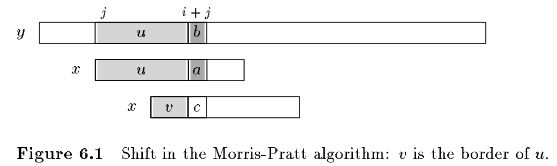
\includegraphics[width=0.8\textwidth]{img151.jpg}
	\caption{Dịch chuyển trong thuật toán Morris-Pratt: $v$ là border của $u$}
\end{figure}

Gọi $\text{mpNext}[i]$ là độ dài của border của $x[0..i-1]$ ($0 < i \leq m$). Thuật toán thực hiện tối đa $2n - 1$ phép so sánh ký tự.

\subsection{Đánh giá độ phức tạp thuật toán}

\begin{itemize}
	\item Pha tiền xử lý: $O(m)$.
	\item Pha tìm kiếm: $O(m + n)$.
\end{itemize}

\subsection{Kiểm nghiệm thuật toán}

Với $x = \texttt{GCAGAGAG}$, $y = \texttt{GCATCGCAGAGAGTATACAGTACG}$:

Bảng $\text{mpNext}[i]$:

\begin{center}
\begin{tabular}{|c|c|c|c|c|c|c|c|c|c|}
\hline
$i$ & 0 & 1 & 2 & 3 & 4 & 5 & 6 & 7 & 8 \\
\hline
$x[i]$ & G & C & A & G & A & G & A & G & \\
\hline
$\text{mpNext}[i]$ & $-1$ & 0 & 0 & 0 & 1 & 0 & 1 & 0 & 1 \\
\hline
\end{tabular}
\end{center}

\begin{figure}[H]
	\centering
	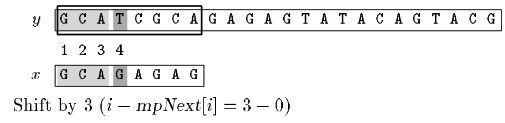
\includegraphics[width=0.9\textwidth]{img153.jpg}
	\caption{Lần 1: Mismatch tại i=3, dịch $i - \text{mpNext}[i] = 3 - 0 = 3$ bước}
\end{figure}
\begin{figure}[H]
	\centering
	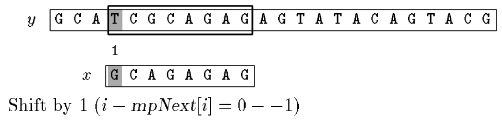
\includegraphics[width=0.9\textwidth]{img154.jpg}
	\caption{Lần 2: Dịch $0 - (-1) = 1$ bước}
\end{figure}
\begin{figure}[H]
	\centering
	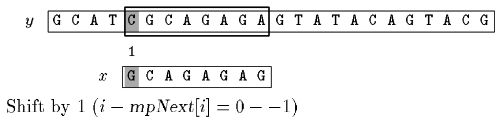
\includegraphics[width=0.9\textwidth]{img157.jpg}
	\caption{Lần 3: Dịch 1 bước}
\end{figure}
\begin{figure}[H]
	\centering
	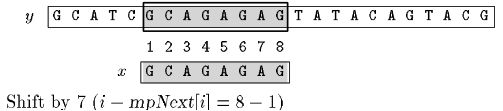
\includegraphics[width=0.9\textwidth]{img158.jpg}
	\caption{Lần 4: Khớp 8 ký tự -- OUTPUT(5), dịch $8 - 1 = 7$ bước}
\end{figure}
\begin{figure}[H]
	\centering
	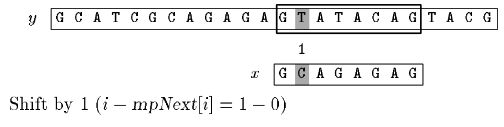
\includegraphics[width=0.9\textwidth]{img159.jpg}
	\caption{Lần 5: Dịch 1 bước}
\end{figure}
\begin{figure}[H]
	\centering
	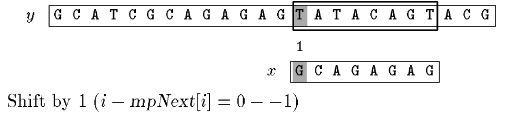
\includegraphics[width=0.9\textwidth]{img160.jpg}
	\caption{Lần 6: Dịch 1 bước}
\end{figure}
\begin{figure}[H]
	\centering
	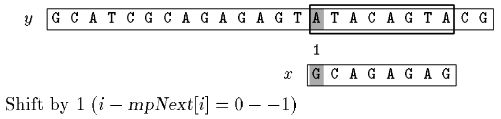
\includegraphics[width=0.9\textwidth]{img161.jpg}
	\caption{Lần 7: Dịch 1 bước}
\end{figure}
\begin{figure}[H]
	\centering
	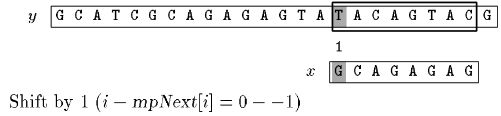
\includegraphics[width=0.9\textwidth]{img162.jpg}
	\caption{Lần 8: Dịch 1 bước}
\end{figure}
\begin{figure}[H]
	\centering
	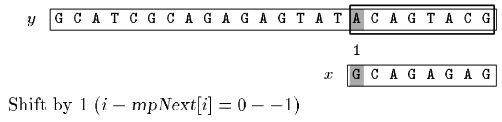
\includegraphics[width=0.9\textwidth]{img165.jpg}
	\caption{Lần 9: Dịch 1 bước}
\end{figure}

Thuật toán Morris-Pratt thực hiện 19 lần so sánh ký tự trong ví dụ trên.

\subsection{Lập trình theo thuật toán}

\begin{lstlisting}[style=CStyle]
void preMp(char *x, int m, int mpNext[]) {
    int i, j;
    i = 0;
    j = mpNext[0] = -1;
    while (i < m) {
        while (j > -1 && x[i] != x[j])
            j = mpNext[j];
        mpNext[++i] = ++j;
    }
}

void MP(char *x, int m, char *y, int n) {
    int i, j, mpNext[XSIZE];
    preMp(x, m, mpNext);
    i = j = 0;
    while (j < n) {
        while (i > -1 && x[i] != y[j])
            i = mpNext[i];
        i++;
        j++;
        if (i >= m) {
            OUTPUT(j - i);
            i = mpNext[i];
        }
    }
}
\end{lstlisting}

%-----------------------------------------------------------
\section{Thuật toán Knuth-Morris-Pratt}
%-----------------------------------------------------------

\subsection{Trình bày thuật toán}

Thuật toán này là một sự cải tiến của thuật toán Morris-Pratt.

Giả sử ta đang đặt cửa sổ tại vị trí $j$ của văn bản $y$ và $x[0..i-1] = y[j..i+j-1] = u$ và $a = x[i] \neq y[i+j] = b$.

\textbf{Định nghĩa tagged border:} Tagged border là phần prefix của mẫu $x$ mà match với phần suffix của $u$ (giống với định nghĩa border của thuật toán Morris-Pratt).

Ta gọi $\text{kmpNext}[i]$ là độ dài của tagged border của $x[0..i-1]$ theo sau bởi ký tự $c$ khác ký tự $x[i]$. Ngược lại thì $\text{kmpNext}[i] = -1$ ($0 < i \leq m$). Khi đó ta có thể tránh việc so sánh $c$ với $y[i+j]$ (vì nếu $c = x[i]$ thì đương nhiên $c \neq y[i+j]$ nên ta không cần so sánh nữa).

\begin{figure}[H]
	\centering
	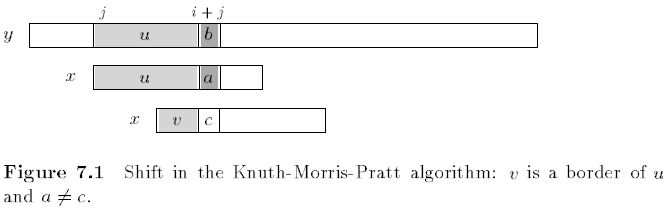
\includegraphics[width=0.8\textwidth]{img171.jpg}
	\caption{Dịch chuyển trong thuật toán Knuth-Morris-Pratt: $v$ là border của $u$ và $a \neq c$}
\end{figure}

\subsection{Đánh giá độ phức tạp thuật toán}

\begin{itemize}
	\item Pha tiền xử lý: $O(m)$.
	\item Pha tìm kiếm: $O(m + n)$.
\end{itemize}

\subsection{Kiểm nghiệm thuật toán}

Với $x = \texttt{GCAGAGAG}$, $y = \texttt{GCATCGCAGAGAGTATACAGTACG}$:

Bảng $\text{kmpNext}[i]$:

\begin{center}
\begin{tabular}{|c|c|c|c|c|c|c|c|c|c|}
\hline
$i$ & 0 & 1 & 2 & 3 & 4 & 5 & 6 & 7 & 8 \\
\hline
$x[i]$ & G & C & A & G & A & G & A & G & \\
\hline
$\text{kmpNext}[i]$ & $-1$ & 0 & 0 & $-1$ & 1 & $-1$ & 1 & $-1$ & 1 \\
\hline
\end{tabular}
\end{center}

\begin{figure}[H]
	\centering
	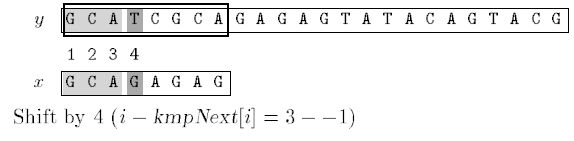
\includegraphics[width=0.9\textwidth]{img173.jpg}
	\caption{Lần 1: Dịch $3 - (-1) = 4$ bước}
\end{figure}
\begin{figure}[H]
	\centering
	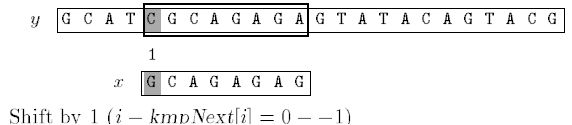
\includegraphics[width=0.9\textwidth]{img174.jpg}
	\caption{Lần 2: Dịch 1 bước}
\end{figure}
\begin{figure}[H]
	\centering
	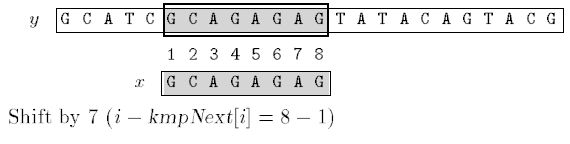
\includegraphics[width=0.9\textwidth]{img177.jpg}
	\caption{Lần 3: OUTPUT(5), dịch 7 bước}
\end{figure}
\begin{figure}[H]
	\centering
	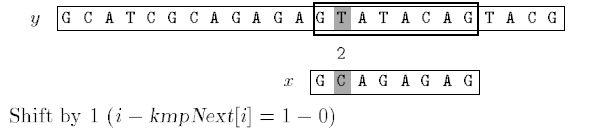
\includegraphics[width=0.9\textwidth]{img178.jpg}
	\caption{Lần 4: Dịch 1 bước}
\end{figure}
\begin{figure}[H]
	\centering
	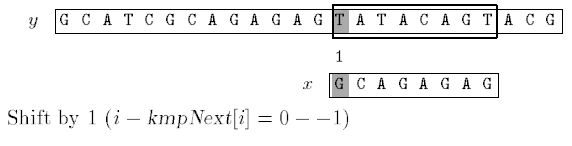
\includegraphics[width=0.9\textwidth]{img179.jpg}
	\caption{Lần 5: Dịch 1 bước}
\end{figure}
\begin{figure}[H]
	\centering
	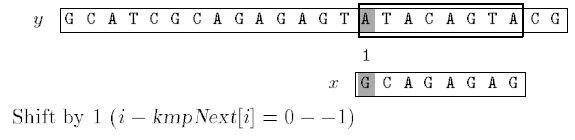
\includegraphics[width=0.9\textwidth]{img180.jpg}
	\caption{Lần 6: Dịch 1 bước}
\end{figure}
\begin{figure}[H]
	\centering
	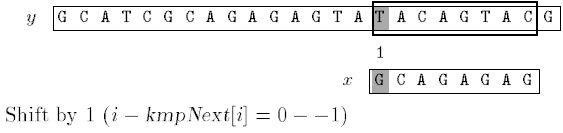
\includegraphics[width=0.9\textwidth]{img181.jpg}
	\caption{Lần 7: Dịch 1 bước}
\end{figure}
\begin{figure}[H]
	\centering
	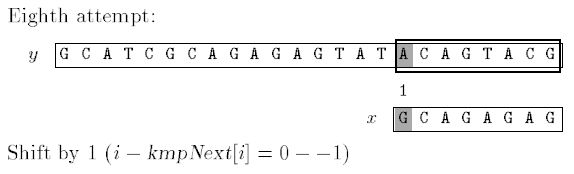
\includegraphics[width=0.9\textwidth]{img182.jpg}
	\caption{Lần 8: Dịch 1 bước}
\end{figure}

Thuật toán KMP thực hiện 18 lần so sánh ký tự trong ví dụ trên.

\subsection{Lập trình theo thuật toán}

\begin{lstlisting}[style=CStyle]
void preKmp(char *x, int m, int kmpNext[]) {
    int i, j;
    i = 0;
    j = kmpNext[0] = -1;
    while (i < m) {
        while (j > -1 && x[i] != x[j])
            j = kmpNext[j];
        i++;
        j++;
        if (x[i] == x[j])
            kmpNext[i] = kmpNext[j];
        else
            kmpNext[i] = j;
    }
}

void KMP(char *x, int m, char *y, int n) {
    int i, j, kmpNext[XSIZE];
    preKmp(x, m, kmpNext);
    i = j = 0;
    while (j < n) {
        while (i > -1 && x[i] != y[j])
            i = kmpNext[i];
        i++;
        j++;
        if (i >= m) {
            OUTPUT(j - i);
            i = kmpNext[i];
        }
    }
}
\end{lstlisting}

%-----------------------------------------------------------
\section{Thuật toán Apostolico-Crochemore}
%-----------------------------------------------------------

\subsection{Trình bày thuật toán}

Thuật toán Apostolico-Crochemore sử dụng bảng $\text{kmpNext}$ trong thuật toán KMP để tính độ dịch chuyển của cửa sổ.

Đặt $\ell = 0$ nếu $x$ là lũy thừa của 1 ký tự ($x = c^m$). Ngược lại, đặt $\ell =$ vị trí của ký tự đầu tiên trong $x$ mà khác $x[0]$. Mỗi lần thử, thuật toán so sánh theo thứ tự: $\ell, \ell+1, \ldots, m-1, 0, 1, \ldots, \ell-1$.

Trong pha tìm kiếm, thuật toán duy trì bộ ba $(i, j, k)$, trong đó:
\begin{itemize}
	\item Cửa sổ được đặt ở đoạn $y[j..j+m-1]$;
	\item $0 \leq k \leq \ell$ và $x[0..k-1] = y[j..j+k-1]$;
	\item $\ell \leq i < m$ và $x[\ell..i-1] = y[j+\ell..i+j-1]$.
\end{itemize}

\begin{figure}[H]
	\centering
	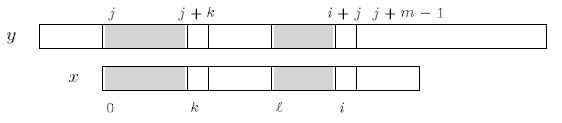
\includegraphics[width=0.8\textwidth]{img190.jpg}
	\caption{Minh họa bộ ba $(i, j, k)$: vùng xám biểu diễn các đoạn đã khớp trong $y$ và $x$}
\end{figure}

Ban đầu bộ ba được khởi tạo $(i, j, k) = (\ell, 0, 0)$. Cách tính bộ ba tiếp theo dựa vào bộ ba trước đó:

\begin{itemize}
	\item \textbf{Trường hợp $i = \ell$:}
	\begin{itemize}
		\item Nếu $x[i] = y[i+j]$ thì bộ ba tiếp theo là $(i+1,\; j,\; k)$.
		\item Nếu $x[i] \neq y[i+j]$ thì bộ ba tiếp theo là $(\ell,\; j+1,\; \max\{0,\, k-1\})$.
	\end{itemize}
	\item \textbf{Trường hợp $\ell < i < m$:}
	\begin{itemize}
		\item Nếu $x[i] = y[i+j]$ thì bộ ba tiếp theo là $(i+1,\; j,\; k)$.
		\item Nếu $x[i] \neq y[i+j]$, xét $\text{kmpNext}[i]$:
		\begin{itemize}
			\item Nếu $\text{kmpNext}[i] \leq \ell$: bộ ba tiếp theo là $\bigl(\ell,\; i+j-\text{kmpNext}[i],\; \max\{0,\, \text{kmpNext}[i]\}\bigr)$.
			\item Nếu $\text{kmpNext}[i] > \ell$: bộ ba tiếp theo là $\bigl(\text{kmpNext}[i],\; i+j-\text{kmpNext}[i],\; \ell\bigr)$.
		\end{itemize}
	\end{itemize}
	\item \textbf{Trường hợp $i = m$:}
	\begin{itemize}
		\item Nếu $k < \ell$ và $x[k] = y[j+k]$ thì bộ ba tiếp theo là $(i,\; j,\; k+1)$.
		\item Ngược lại (hoặc $k = \ell$): nếu $k = \ell$ thì thông báo tìm thấy mẫu tại vị trí $j$. Trong cả hai trường hợp, bộ ba tiếp theo được tính như trong trường hợp $\ell < i < m$.
	\end{itemize}
\end{itemize}

\subsection{Đánh giá độ phức tạp thuật toán}

\begin{itemize}
	\item Pha tiền xử lý: $O(m)$.
	\item Pha tìm kiếm: $O(n)$.
\end{itemize}

\subsection{Kiểm nghiệm thuật toán}

Bảng $\text{kmpNext}$ với $x = \texttt{GCAGAGAG}$, $\ell = 1$:

\begin{center}
\begin{tabular}{|c|c|c|c|c|c|c|c|c|c|}
\hline
$i$ & 0 & 1 & 2 & 3 & 4 & 5 & 6 & 7 & 8 \\
\hline
$x[i]$ & G & C & A & G & A & G & A & G & \\
\hline
$\text{kmpNext}[i]$ & $-1$ & 0 & 0 & $-1$ & 1 & $-1$ & 1 & $-1$ & 1 \\
\hline
\end{tabular}
\end{center}

\begin{figure}[H]
	\centering
	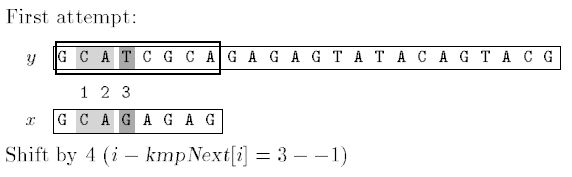
\includegraphics[width=0.9\textwidth]{img194.jpg}
	\caption{Lần 1: Dịch 4 bước}
\end{figure}
\begin{figure}[H]
	\centering
	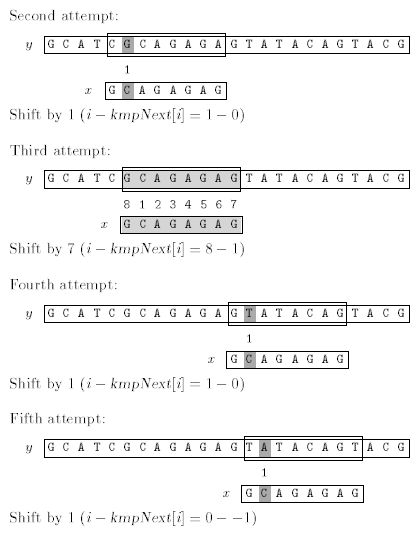
\includegraphics[width=0.9\textwidth]{img195.jpg}
	\caption{Lần 2: Dịch 1 bước; lần 3: OUTPUT(5), dịch 7 bước; lần 4--5: Dịch 1 bước}
\end{figure}
\begin{figure}[H]
	\centering
	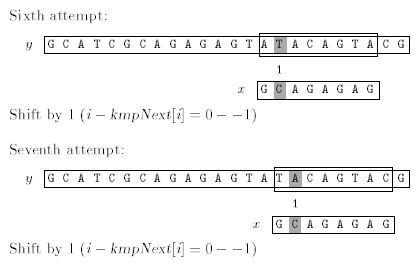
\includegraphics[width=0.9\textwidth]{img198.jpg}
	\caption{Lần 6--7: Dịch 1 bước}
\end{figure}
\begin{figure}[H]
	\centering
	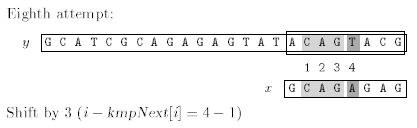
\includegraphics[width=0.9\textwidth]{img199.jpg}
	\caption{Lần 8: Dịch 3 bước}
\end{figure}

Thuật toán Apostolico-Crochemore thực hiện 20 phép so sánh ký tự trong ví dụ trên.

\subsection{Lập trình theo thuật toán}

\begin{lstlisting}[style=CStyle]
void AC(char *x, int m, char *y, int n) {
    int i, j, k, ell, kmpNext[XSIZE];
    preKmp(x, m, kmpNext);
    for (ell = 1; ell < m && x[ell - 1] == x[ell]; ell++);
    if (ell == m) ell = 0;
    i = ell;
    j = k = 0;
    while (j <= n - m) {
        while (i < m && x[i] == y[i + j])
            ++i;
        if (i >= m) {
            while (k < ell && x[k] == y[j + k])
                ++k;
            if (k >= ell)
                OUTPUT(j);
        }
        if (i == ell || kmpNext[i] <= ell) {
            j += (i - kmpNext[i]);
            i = ell;
            k = (k > 0) ? k - 1 : 0;
        } else {
            j += (i - kmpNext[i]);
            k = (kmpNext[i] > ell) ? ell : kmpNext[i];
            i = kmpNext[i];
        }
    }
}
\end{lstlisting}

%-----------------------------------------------------------
\section{Thuật toán Not So Naïve}
%-----------------------------------------------------------

\subsection{Trình bày thuật toán}

Trong pha tìm kiếm của thuật toán Not So Naïve, việc so sánh các ký tự của mẫu $x$ được thực hiện theo thứ tự: $1, 2, \ldots, m-2, m-1, 0$.

Mỗi lần thử (tức mỗi lần đặt cửa sổ vào đoạn $y[j..j+m-1]$ của văn bản $y$):
\begin{itemize}
	\item Nếu $x[0] = x[1]$ và $x[1] \neq y[j+1]$ (suy ra $x[0] \neq y[j+1]$), hoặc nếu $x[0] \neq x[1]$ và $x[1] = y[j+1]$ (suy ra $x[0] \neq y[j+1]$): thì cửa sổ được dịch \textbf{2 vị trí}.
	\item Ngược lại: cửa sổ được dịch \textbf{1 vị trí}.
\end{itemize}

Ta thấy thuật toán Not So Naïve gần giống với thuật toán Brute Force nhưng có cải tiến một chút (vì vậy mới có tên là Not So Naïve).

\subsection{Đánh giá độ phức tạp thuật toán}

\begin{itemize}
	\item Pha tiền xử lý: độ phức tạp hằng số.
	\item Pha tìm kiếm: $O(m \times n)$.
\end{itemize}

\subsection{Kiểm nghiệm thuật toán}

\begin{figure}[H]
	\centering
	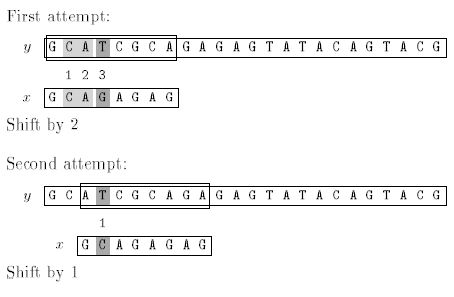
\includegraphics[width=0.9\textwidth]{img206.jpg}
	\caption{Lần 1: Dịch 2 bước; lần 2: Dịch 1 bước}
\end{figure}
\begin{figure}[H]
	\centering
	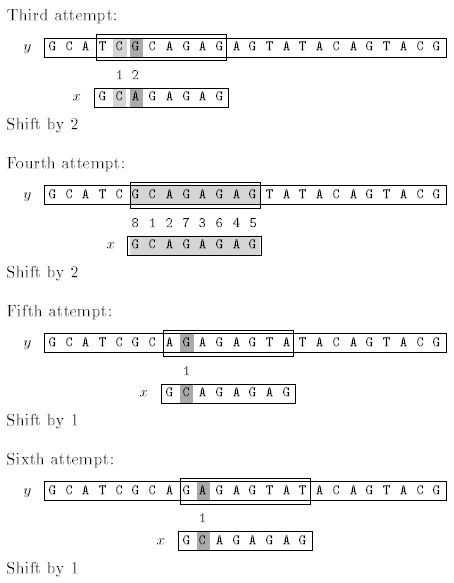
\includegraphics[width=0.9\textwidth]{img207.jpg}
	\caption{Lần 3--4: Dịch 2 bước; lần 5--6: Dịch 1 bước}
\end{figure}
\begin{figure}[H]
	\centering
	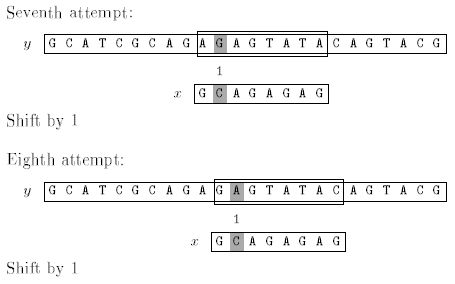
\includegraphics[width=0.9\textwidth]{img210.jpg}
	\caption{Lần 7--8: Dịch 1 bước}
\end{figure}
\begin{figure}[H]
	\centering
	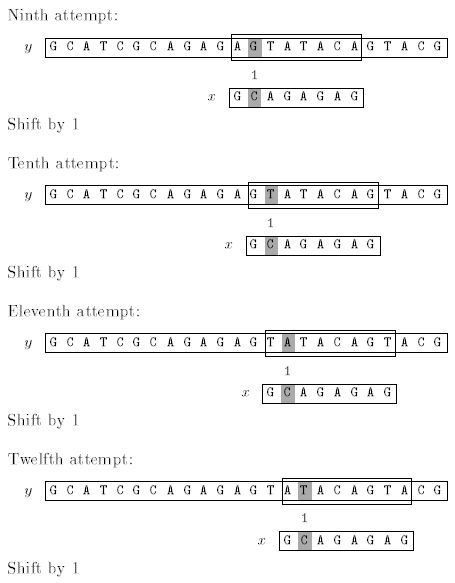
\includegraphics[width=0.9\textwidth]{img211.jpg}
	\caption{Lần 9--12: Dịch 1 bước}
\end{figure}
\begin{figure}[H]
	\centering
	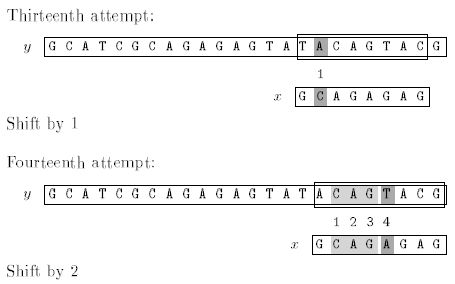
\includegraphics[width=0.9\textwidth]{img214.jpg}
	\caption{Lần 13: Dịch 1 bước; lần 14: Dịch 2 bước}
\end{figure}

Ta thấy thuật toán Not So Naïve thực hiện 27 phép so sánh ký tự trong ví dụ trên.

\subsection{Lập trình theo thuật toán}

\begin{lstlisting}[style=CStyle]
void NSN(char *x, int m, char *y, int n) {
    int j, k, ell;
    if (x[0] == x[1]) { k = 2; ell = 1; }
    else               { k = 1; ell = 2; }
    j = 0;
    while (j <= n - m) {
        if (x[1] != y[j + 1])
            j += k;
        else {
            if (memcmp(x + 2, y + j + 2, m - 2) == 0 &&
                x[0] == y[j])
                OUTPUT(j);
            j += ell;
        }
    }
}
\end{lstlisting}

%=============================================================
\chapter{Tìm kiếm mẫu từ phải sang trái}
%=============================================================

\section{Thuật toán Boyer-Moore}

\subsection{Trình bày thuật toán}

Thuật toán Boyer-Moore so sánh các ký tự của pattern $x$ với văn bản $y$ từ phải sang trái và dựa trên 2 kiểu dịch chuyển cửa sổ là good-suffix shift và bad-character shift.

\textbf{Good-suffix shift:} Giả sử sự không khớp xảy ra ở cặp $a = x[i]$ và $y[i+j] = b$ trong lần thử ở vị trí $j$ của văn bản $y$. Do đó $x[i+1..m-1] = y[i+j+1..j+m-1] = u$ và $x[i] \neq y[i+j]$. Good-suffix shift dùng thẳng đoạn $y[i+j+1..j+m-1] = x[i+1..m-1] = u$ với 1 segment bên phải nhất của $x$ sao cho segment đó $= u$ và ký tự ngay trước nó khác $x[i]$. Nếu không có một segment nào như vậy thì sẽ dịch cửa sổ sao cho dùng thẳng suffix dài nhất $v$ của đoạn $y[i+j+1..j+m-1]$ với một prefix của $x$ mà match với suffix đó.

\begin{figure}[H]
	\centering
	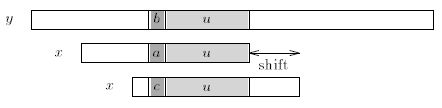
\includegraphics[width=0.8\textwidth]{img217.jpg}
	\caption{Good-suffix shift trong trường hợp tìm được 1 segment trong $x$ mà ký tự $c$ ngay trước nó khác $a$}
\end{figure}

\begin{figure}[H]
	\centering
	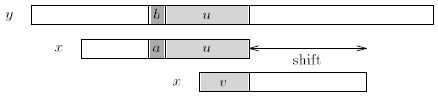
\includegraphics[width=0.8\textwidth]{img218.jpg}
	\caption{Good-suffix shift trong trường hợp không tìm được segment trong $x$ thỏa mãn yêu cầu}
\end{figure}

\textbf{Bad-character shift:} Dùng ký tự $y[i+j] = b$ của văn bản $y$ với 1 ký tự $c$ bên phải nhất của đoạn $x[0..m-2]$ sao cho $c = b$. Nếu không tìm thấy ký tự $b = y[i+j]$ trong mẫu $x$ thì ta dịch cửa sổ ra ngay sau ký tự $b$ tức cửa sổ bắt đầu ở ký tự $y[i+j+1]$.

\begin{figure}[H]
	\centering
	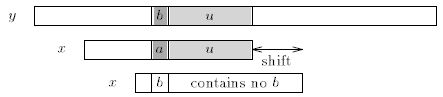
\includegraphics[width=0.8\textwidth]{img219.jpg}
	\caption{Bad-character shift trong trường hợp tìm thấy một ký tự $b$ trong $x$ thỏa mãn yêu cầu}
\end{figure}

\begin{figure}[H]
	\centering
	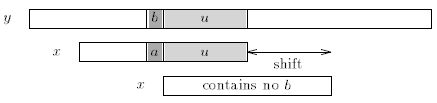
\includegraphics[width=0.8\textwidth]{img220.jpg}
	\caption{Bad-character shift trong trường hợp không tìm thấy ký tự $b$ trong $x$}
\end{figure}

Với mỗi lần thử ta có 2 cách dịch chuyển cửa sổ là good-suffix shift và bad-character shift. Đối với bad-character shift, cửa sổ có thể bị dịch lại (dịch sang trái). Ta sẽ chọn cách dịch chuyển mà dịch cửa sổ sang phải nhiều nhất.

\subsection{Đánh giá độ phức tạp thuật toán}

\begin{itemize}
	\item Pha tiền xử lý: $O(m + \sigma)$.
	\item Pha tìm kiếm: $O(m \times n)$ trường hợp xấu nhất, $O(n/m)$ trường hợp trung bình.
\end{itemize}

\subsection{Kiểm nghiệm thuật toán}

Với $x = \texttt{GCAGAGAG}$, $y = \texttt{GCATCGCAGAGAGTATACAGTACG}$:

\begin{center}
\begin{tabular}{|c|c|c|c|c|}
\hline
$a$ & A & C & G & T \\
\hline
\texttt{bmBc} & 1 & 6 & 2 & 8 \\
\hline
\end{tabular}
\end{center}

\begin{center}
\begin{tabular}{|c|c|c|c|c|c|c|c|c|}
\hline
$i$ & 0 & 1 & 2 & 3 & 4 & 5 & 6 & 7 \\
\hline
$x[i]$ & G & C & A & G & A & G & A & G \\
\hline
$\text{suff}[i]$ & 1 & 0 & 0 & 2 & 0 & 4 & 0 & 8 \\
\hline
$\text{bmGs}[i]$ & 7 & 7 & 7 & 2 & 7 & 4 & 7 & 1 \\
\hline
\end{tabular}
\end{center}

\begin{figure}[H]
	\centering
	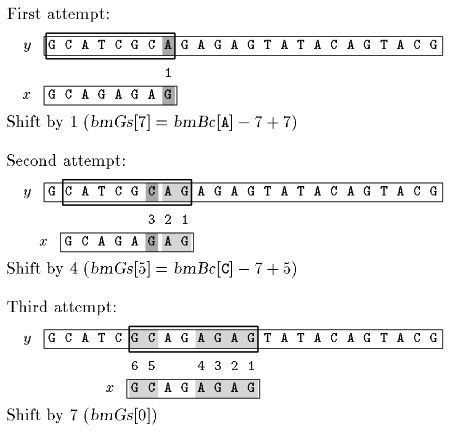
\includegraphics[width=0.9\textwidth]{img242.jpg}
	\caption{Lần 1--3: Lần 3 OUTPUT(5)}
\end{figure}
\begin{figure}[H]
	\centering
	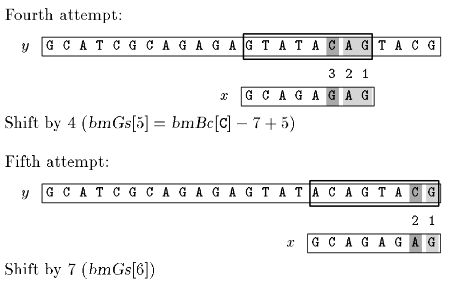
\includegraphics[width=0.9\textwidth]{img243.jpg}
	\caption{Lần 4--5: Kết thúc}
\end{figure}

Ta thấy thuật toán Boyer-Moore thực hiện 17 phép so sánh ký tự trong ví dụ trên.

\subsection{Lập trình theo thuật toán}

\begin{lstlisting}[style=CStyle]
void preBmGs(char *x, int m, int bmGs[]) {
    int i, j, suff[XSIZE];
    suffixes(x, m, suff);
    for (i = 0; i < m; ++i)
        bmGs[i] = m;
    j = 0;
    for (i = m - 1; i >= 0; --i)
        if (suff[i] == i + 1)
            for (; j < m - 1 - i; ++j)
                if (bmGs[j] == m)
                    bmGs[j] = m - 1 - i;
    for (i = 0; i <= m - 2; ++i)
        bmGs[m - 1 - suff[i]] = m - 1 - i;
}

void BM(char *x, int m, char *y, int n) {
    int i, j, bmGs[XSIZE], bmBc[ASIZE];
    preBmGs(x, m, bmGs);
    preBmBc(x, m, bmBc);
    j = 0;
    while (j <= n - m) {
        for (i = m - 1; i >= 0 && x[i] == y[i + j]; --i);
        if (i < 0) {
            OUTPUT(j);
            j += bmGs[0];
        } else
            j += MAX(bmGs[i],
                     bmBc[(unsigned char)y[i+j]] - m + 1 + i);
    }
}
\end{lstlisting}

%-----------------------------------------------------------
\section{Thuật toán Turbo-BM}
%-----------------------------------------------------------

\subsection{Trình bày thuật toán}

Thuật toán Turbo-BM là sự cải tiến của thuật toán Boyer-Moore. Thuật toán này cốt yếu ở việc nó ghi nhớ đoạn text của $y$ (chính là đoạn $u$ trong thuật toán Boyer-Moore) mà match với suffix của $x$ ở lần thử trước đó (chỉ khi một good-suffix shift được thực hiện). Kỹ thuật này có 2 lợi thế:
\begin{itemize}
	\item Nó có thể nhảy qua đoạn text đó (đoạn $u$).
	\item Nó cho phép thực hiện một turbo-shift.
\end{itemize}

\textbf{Định nghĩa turbo-shift:} Turbo-shift chỉ có thể xuất hiện nếu ở lần thử hiện tại suffix của pattern mà match với text là ngắn hơn suffix ở lần thử trước đó. Trong trường hợp này chúng ta gọi $u$ là suffix trước đó và $v$ là suffix ở lần thử hiện tại. Gọi $a$ và $b$ là các ký tự gây ra sự không khớp (mismatch) trong lần thử hiện tại ($a$ thuộc $x$ và $b$ thuộc $y$). Thì $av$ là suffix của $x$ và $av$ cũng là suffix của $u$ (do độ dài $v$ bé hơn độ dài $u$). Hai ký tự $a$ và $b$ cách nhau khoảng cách $p$ trong text, và suffix của $x$ có độ dài $|uzv|$ có 1 đoạn độ dài $p = |zv|$. Vì $u$ là border của $uzv$ $\Rightarrow$ sẽ không tìm thấy $x$ trong $y$ khi ký tự $b$ chạy sang trái 1 đoạn $|u| - |v| - 1$. Vậy độ dịch nhỏ nhất có thể có độ dài là $|u| - |v|$, ta gọi nó là turbo-shift.

\begin{figure}[H]
	\centering
	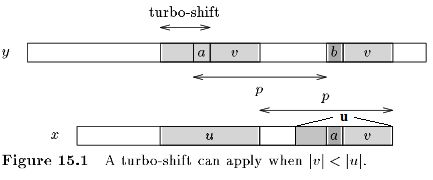
\includegraphics[width=0.8\textwidth]{img236.jpg}
	\caption{Turbo-shift khi $|v| < |u|$}
\end{figure}

Xét trường hợp $|v| < |u|$, nếu độ dài của bad-character shift lớn hơn độ dài của good-suffix shift và turbo-shift thì độ dài dịch chuyển cửa sổ thực sự phải là $|u| + 1$. Thật vậy, trong trường hợp này 2 ký tự $c$ và $d$ là khác nhau và ta đang giả sử rằng lần dịch trước là good-suffix shift. Thì sau đó một sự dịch chuyển dài hơn turbo-shift nhưng ngắn hơn $|u| + 1$ sẽ dùng $c$ và $d$ vào vị trí với cùng một ký tự trong $v$, do vậy sẽ không tìm thấy một sự match nào. Do đó, trường hợp này độ dài dịch chuyển thực sự ít nhất phải bằng $|u| + 1$.

\begin{figure}[H]
	\centering
	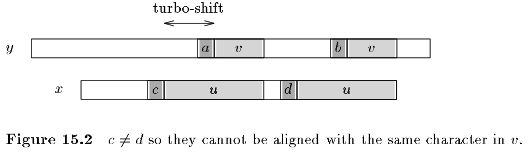
\includegraphics[width=0.8\textwidth]{img237.jpg}
	\caption{Turbo-shift: $c \neq d$ không thể căn chỉnh với cùng ký tự trong $v$}
\end{figure}

Như vậy ta thấy rằng nếu $|v| \geq |u|$, ta so sánh good-suffix shift và bad-character shift để chọn ra cái tốt nhất. Ngược lại nếu $|v| < |u|$, ta so sánh turbo-shift, good-suffix shift, bad-character shift và $|u|+1$ để chọn ra cái tốt nhất.

\subsection{Đánh giá độ phức tạp thuật toán}

\begin{itemize}
	\item Pha tiền xử lý: $O(m + \sigma)$.
	\item Pha tìm kiếm: $O(n)$.
\end{itemize}

\subsection{Kiểm nghiệm thuật toán}

Với $x = \texttt{GCAGAGAG}$, $y = \texttt{GCATCGCAGAGAGTATACAGTACG}$:

\begin{center}
\begin{tabular}{|c|c|c|c|c|}
\hline
$a$ & A & C & G & T \\
\hline
$\text{qsBc}[a]$ & 2 & 7 & 1 & 9 \\
\hline
\end{tabular}
\end{center}

\begin{figure}[H]
	\centering
	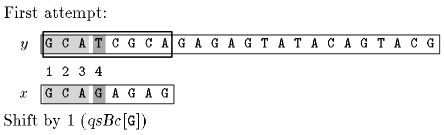
\includegraphics[width=0.9\textwidth]{img251.jpg}
	\caption{Lần 1: Dịch 3 bước}
\end{figure}
\begin{figure}[H]
	\centering
	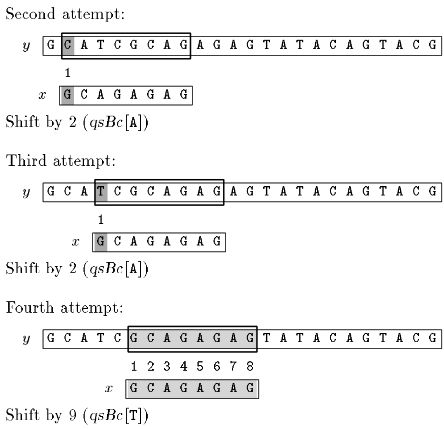
\includegraphics[width=0.9\textwidth]{img252.jpg}
	\caption{Lần 2: Dịch 2 bước; lần 3: Dịch 2 bước; lần 4: OUTPUT(5), dịch 9 bước}
\end{figure}
\begin{figure}[H]
	\centering
	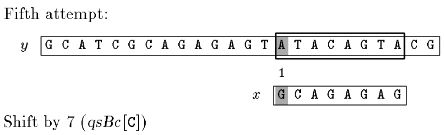
\includegraphics[width=0.9\textwidth]{img257.jpg}
	\caption{Lần 5: Dịch 7 bước}
\end{figure}

Ta thấy thuật toán Turbo-Boyer-Moore thực hiện 15 phép so sánh ký tự trong ví dụ trên.

\subsection{Lập trình theo thuật toán}

\begin{lstlisting}[style=CStyle]
void TBM(char *x, int m, char *y, int n) {
    int bcShift, i, j, shift, u, v, turboShift;
    int bmGs[XSIZE], bmBc[ASIZE];
    preBmGs(x, m, bmGs);
    preBmBc(x, m, bmBc);
    j = u = 0;
    shift = m;
    while (j <= n - m) {
        i = m - 1;
        while (i >= 0 && x[i] == y[i + j]) {
            --i;
            if (u != 0 && i == m - 1 - shift)
                i -= u;
        }
        if (i < 0) {
            OUTPUT(j);
            shift = bmGs[0];
            u = m - shift;
        } else {
            v = m - 1 - i;
            turboShift = u - v;
            bcShift = bmBc[(unsigned char)y[i+j]] - m + 1 + i;
            shift = MAX(turboShift, bcShift);
            shift = MAX(shift, bmGs[i]);
            if (shift == bmGs[i])
                u = MIN(m - shift, v);
            else {
                if (turboShift < bcShift)
                    shift = MAX(shift, u + 1);
                u = 0;
            }
        }
        j += shift;
    }
}
\end{lstlisting}

%-----------------------------------------------------------
\section{Thuật toán Quick Search}
%-----------------------------------------------------------

\subsection{Trình bày thuật toán}

Là phiên bản đơn giản hóa của thuật toán Boyer-Moore. Chỉ sử dụng bad-character shift. Dễ dàng cài đặt.

Ta thấy rằng sau mỗi lần thử (tức cửa sổ được đặt ở đoạn $y[j..j+m-1]$ của text), độ dài dịch chuyển ít nhất phải bằng 1, vậy nên ký tự $y[j+m]$ đương nhiên sẽ được xét trong lần thử tiếp theo. Và vì vậy $y[j+m]$ có thể được sử dụng cho bad-character shift của lần thử hiện tại. Bad-character shift của thuật toán này được sửa đổi một chút như sau:

\[
\text{qsBc}[c] = \begin{cases}
\min\{m - i : 0 \leq i < m-1,\ x[i] = c\} + 1 & \text{nếu } c \in x \\
m + 1 & \text{nếu } c \notin x
\end{cases}
\]

Như vậy trong mỗi lần thử tại đoạn $y[j..j+m-1]$, nếu không match với pattern $x$ ta tìm bad-character shift với bad-character shift $= \text{qsBc}[y[j+m]]$.

\subsection{Đánh giá độ phức tạp thuật toán}

\begin{itemize}
	\item Pha tiền xử lý: độ phức tạp thời gian $O(m + \sigma)$ và độ phức tạp bộ nhớ $O(\sigma)$.
	\item Pha tìm kiếm có độ phức tạp thời gian là $O(m \times n)$.
\end{itemize}

\subsection{Kiểm nghiệm thuật toán}

Bảng qsBc cho $x = \texttt{GCAGAGAG}$:
\begin{center}
\begin{tabular}{|c|c|c|c|c|}
\hline
$a$ & A & C & G & T \\
\hline
\texttt{qsBc} & 2 & 7 & 1 & 9 \\
\hline
\end{tabular}
\end{center}

\begin{figure}[H]
	\centering
	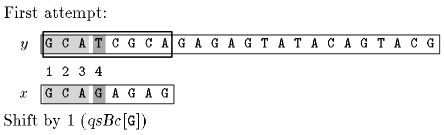
\includegraphics[width=0.9\textwidth]{img251.jpg}
	\caption{Lần 1: Dịch 1 (qsBc[G])}
\end{figure}
\begin{figure}[H]
	\centering
	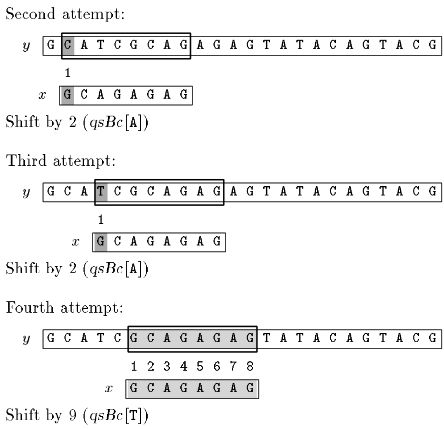
\includegraphics[width=0.9\textwidth]{img252.jpg}
	\caption{Lần 2--4: OUTPUT(5) ở lần 4, dịch 9 (qsBc[T])}
\end{figure}
\begin{figure}[H]
	\centering
	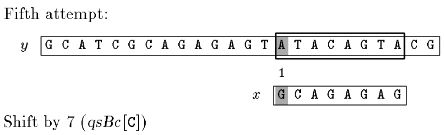
\includegraphics[width=0.9\textwidth]{img257.jpg}
	\caption{Lần 5: Kết thúc}
\end{figure}

Ta thấy thuật toán Quick Search thực hiện 15 phép so sánh ký tự trong ví dụ trên.

\subsection{Lập trình theo thuật toán}

\begin{lstlisting}[style=CStyle]
void preQsBc(char *x, int m, int qsBc[]) {
    int i;
    for (i = 0; i < ASIZE; ++i)
        qsBc[i] = m + 1;
    for (i = 0; i < m; ++i)
        qsBc[(unsigned char)x[i]] = m - i;
}

void QS(char *x, int m, char *y, int n) {
    int j, qsBc[ASIZE];
    preQsBc(x, m, qsBc);
    j = 0;
    while (j <= n - m) {
        if (memcmp(x, y + j, m) == 0)
            OUTPUT(j);
        if (j + m < n)
            j += qsBc[(unsigned char)y[j + m]];
        else
            break;
    }
}
\end{lstlisting}

%-----------------------------------------------------------
\section{Thuật toán Tuned Boyer-Moore}
%-----------------------------------------------------------

\subsection{Trình bày thuật toán}

Tuned-Boyer-Moore là phiên bản đơn giản hóa của thuật toán Boyer-Moore, dễ cài đặt và rất nhanh trong thực tế.

Phần tốn chi phí nhất trong các thuật toán đối sánh mẫu là kiểm tra xem liệu ký tự trong mẫu có khớp với ký tự trong cửa sổ không. Để tránh việc kiểm tra này nhiều lần, Tuned-Boyer-Moore sẽ dịch chuyển cửa sổ một số lần trước khi thực sự so sánh ký tự.

Thuật toán sử dụng bad-character shift để tìm ký tự $x[m-1]$ trong $y$. Thuật toán sẽ tiếp tục dịch chuyển cửa sổ cho đến khi tìm thấy $x[m-1]$ trong $y$. Thuật toán yêu cầu lưu giá trị của $\text{bmBc}[x[m-1]]$ vào biến \texttt{shift}, và sau đó đặt lại $\text{bmBc}[x[m-1]] = 0$. Khi $x[m-1]$ được tìm thấy trong $y$, $m-1$ ký tự còn lại được kiểm tra và sau đó dịch cửa sổ một đoạn \texttt{shift}.

\subsection{Đánh giá độ phức tạp thuật toán}

\begin{itemize}
	\item Độ phức tạp thuật toán: $O(m \times n)$.
\end{itemize}

\subsection{Kiểm nghiệm thuật toán}

Với $x = \texttt{GCAGAGAG}$, $y = \texttt{GCATCGCAGAGAGTATACAGTACG}$, $\texttt{shift} = 2$:

\begin{center}
\begin{tabular}{|c|c|c|c|c|}
\hline
$a$ & A & C & G & T \\
\hline
$\text{bmBc}[a]$ & 1 & 6 & 0 & 8 \\
\hline
\end{tabular}
\end{center}

\begin{figure}[H]
	\centering
	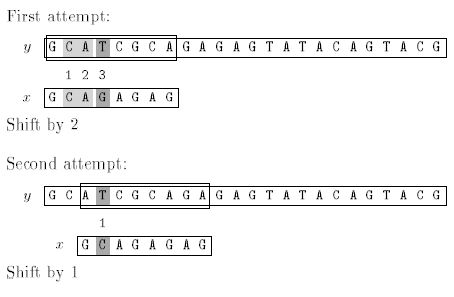
\includegraphics[width=0.9\textwidth]{img206.jpg}
	\caption{Bảng preBmBc và các bước tìm kiếm}
\end{figure}
\begin{figure}[H]
	\centering
	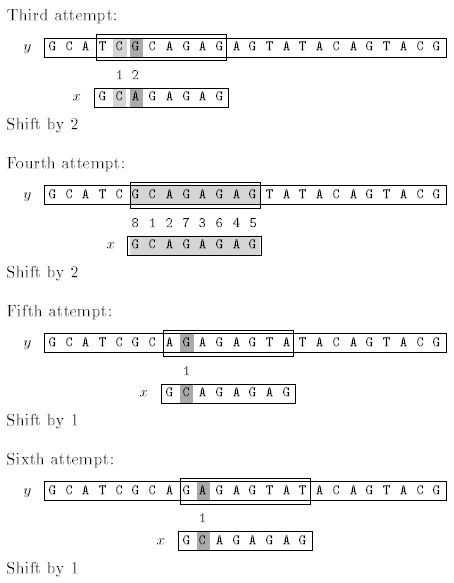
\includegraphics[width=0.9\textwidth]{img207.jpg}
	\caption{OUTPUT(5)}
\end{figure}

\subsection{Lập trình theo thuật toán}

\begin{lstlisting}[style=CStyle]
void TUNEDBM(char *x, int m, char *y, int n) {
    int j, k, shift, bmBc[ASIZE];
    preBmBc(x, m, bmBc);
    shift = bmBc[(unsigned char)x[m - 1]];
    bmBc[(unsigned char)x[m - 1]] = 0;
    memset(y + n, x[m - 1], m);
    j = 0;
    while (j <= n - m) {
        k = bmBc[(unsigned char)y[j + m - 1]];
        while (k != 0) {
            j += k;  k = bmBc[(unsigned char)y[j + m - 1]];
            j += k;  k = bmBc[(unsigned char)y[j + m - 1]];
            j += k;  k = bmBc[(unsigned char)y[j + m - 1]];
        }
        if (memcmp(x, y + j, m - 1) == 0 && j <= n - m)
            OUTPUT(j);
        j += shift;
    }
}
\end{lstlisting}

%-----------------------------------------------------------
\section{Thuật toán Zhu-Takaoka}
%-----------------------------------------------------------

\subsection{Trình bày thuật toán}

Thuật toán Zhu-Takaoka là biến thể của thuật toán Boyer-Moore. Thuật toán sử dụng 2 ký tự liên tiếp nhau để tính bad-character shift. Trong pha tìm kiếm, các so sánh được thực hiện từ phải sang trái trong cửa sổ $y[j..j+m-1]$, và sự không khớp xảy ra ở $x[m-k]$ và $y[j+m-k]$, và đoạn khớp là $x[m-k+1..m-1] = y[j+m-k+1..j+m-1]$. Thuật toán sẽ tính bad-character shift cho 2 ký tự cuối của cửa sổ là $y[j+m-2]$ và $y[j+m-1]$, đồng thời cũng tính được good-suffix shift. Độ dịch lớn hơn sẽ được chọn để dịch cửa sổ ($\max(\text{bad-character shift}, \text{good-suffix shift})$).

Công thức tính bad-character shift cho 2 ký tự $a, b$:
\begin{itemize}
	\item $k < m-2$: $x[m-k..m-k+1] = ab$ và $ab$ không xuất hiện trong $x[m-k+2..m-2]$
	\item $k = m-1$: $x[0] = b$ và $ab$ không xuất hiện trong $x[0..m-2]$
	\item $k = m$: $x[0] \neq b$ và $ab$ không xuất hiện trong $x[0..m-2]$
\end{itemize}

\subsection{Đánh giá độ phức tạp thuật toán}

\begin{itemize}
	\item Pha cài đặt: $O(m + \sigma^2)$.
	\item Pha thực thi: $O(m \times n)$.
\end{itemize}

\subsection{Kiểm nghiệm thuật toán}

Bảng ztBc cho $x = \texttt{GCAGAGAG}$:
\begin{center}
\begin{tabular}{|c|c|c|c|c|}
\hline
\texttt{ztBc} & A & C & G & T \\
\hline
A & 8 & 8 & 2 & 8 \\
C & 5 & 8 & 7 & 8 \\
G & 1 & 6 & 7 & 8 \\
T & 8 & 8 & 7 & 8 \\
\hline
\end{tabular}
\end{center}

\begin{figure}[H]
	\centering
	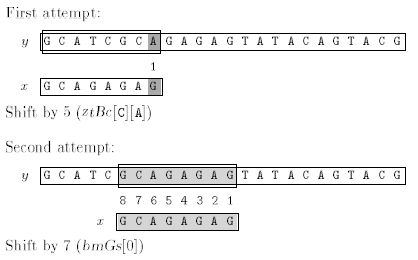
\includegraphics[width=0.9\textwidth]{img272.jpg}
	\caption{Lần 1: Dịch 5 (ztBc[C][A]); Lần 2: OUTPUT(5) dịch 7}
\end{figure}
\begin{figure}[H]
	\centering
	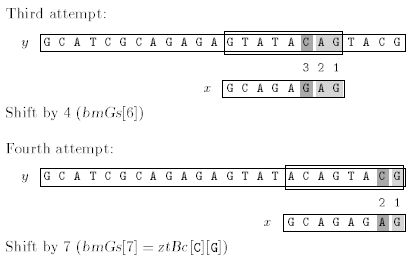
\includegraphics[width=0.9\textwidth]{img273.jpg}
	\caption{Lần 3--4: Kết thúc}
\end{figure}

\subsection{Lập trình theo thuật toán}

\begin{lstlisting}[style=CStyle]
void preZtBc(char *x, int m, int ztBc[][ASIZE]) {
    int i, j;
    for (i = 0; i < ASIZE; ++i)
        for (j = 0; j < ASIZE; ++j)
            ztBc[i][j] = m;
    for (i = 0; i < ASIZE; ++i)
        ztBc[i][(unsigned char)x[0]] = m - 1;
    for (i = 1; i < m - 1; ++i)
        ztBc[(unsigned char)x[i-1]][(unsigned char)x[i]] = m-1-i;
}

void ZT(char *x, int m, char *y, int n) {
    int i, j, ztBc[ASIZE][ASIZE], bmGs[XSIZE];
    preZtBc(x, m, ztBc);
    preBmGs(x, m, bmGs);
    j = 0;
    while (j <= n - m) {
        for (i = m - 1; i >= 0 && x[i] == y[i + j]; --i);
        if (i < 0) {
            OUTPUT(j);
            j += bmGs[0];
        } else
            j += MAX(bmGs[i],
                     ztBc[(unsigned char)y[j+m-2]]
                         [(unsigned char)y[j+m-1]]);
    }
}
\end{lstlisting}

%-----------------------------------------------------------
\section{Thuật toán Berry-Ravindran}
%-----------------------------------------------------------

\subsection{Trình bày thuật toán}

Thuật toán Berry-Ravindran là thuật toán lai giữa 2 thuật toán Quick Search và Zhu-Takaoka. Thuật toán tính bad-character shift cho 2 ký tự liên tiếp nhau nằm ngay sau cửa sổ (là 2 ký tự $y[j+m]$ và $y[j+m+1]$).

Pha tiền xử lý thực hiện tính độ dịch bad-character shift cho cặp ký tự $(a, b)$ với $a, b \in \Sigma$. Cặp $(a, b)$ chính là cặp $(y[j+m], y[j+m+1])$. Ta đặt mẫu $x$ vào giữa $a, b$ (tức $axb$) và tìm sự xuất hiện bên phải nhất của $ab$ trong $axb \Rightarrow$ từ đó tính được giá trị của bad-character shift cho $(a, b)$.

Cách tính bad-character shift cho $(a, b)$:
\[
\text{brBc}[a, b] = \min \begin{cases}
m - 1 - i : x[i] = a,\ x[i+1] = b,\ 0 \leq i < m-1 \\
m : x[0] = b,\ m + 1 : \text{ngược lại}
\end{cases}
\]

Nếu cửa sổ hiện tại đang ở vị trí $y[j..j+m-1]$ thì bước dịch cửa sổ tiếp theo sẽ có độ dài là $\text{brBc}[y[j+m], y[j+m+1]]$.

\subsection{Đánh giá độ phức tạp thuật toán}

\begin{itemize}
	\item Pha tiền xử lý: $O(m + \sigma^2)$.
	\item Pha tìm kiếm: $O(m \times n)$.
\end{itemize}

\subsection{Kiểm nghiệm thuật toán}

Bảng brBc cho $x = \texttt{GCAGAGAG}$:

\begin{center}
\begin{tabular}{|c|c|c|c|c|c|}
\hline
\texttt{brBc} & A & C & G & T & * \\
\hline
A  & 10 & 10 & 2  & 10 & 10 \\
C  & 7  & 10 & 9  & 10 & 10 \\
G  & 1  & 1  & 1  & 1  & 1  \\
T  & 10 & 10 & 9  & 10 & 10 \\
*  & 10 & 10 & 9  & 10 & 10 \\
\hline
\end{tabular}
\end{center}

\begin{figure}[H]
	\centering
	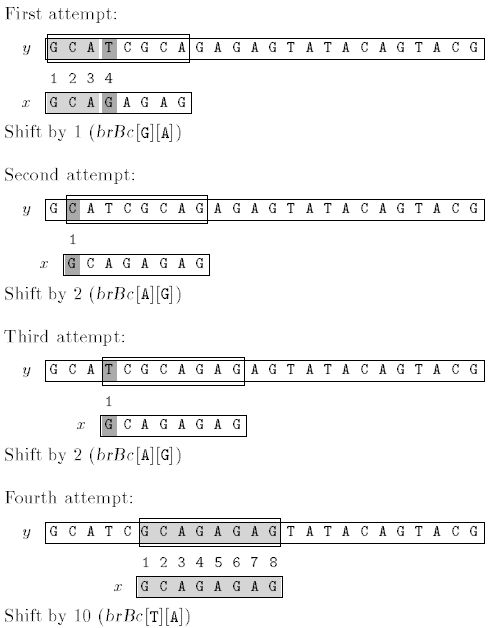
\includegraphics[width=0.9\textwidth]{img282.jpg}
	\caption{Lần 1--4: Lần 4 OUTPUT(5), dịch 10}
\end{figure}
\begin{figure}[H]
	\centering
	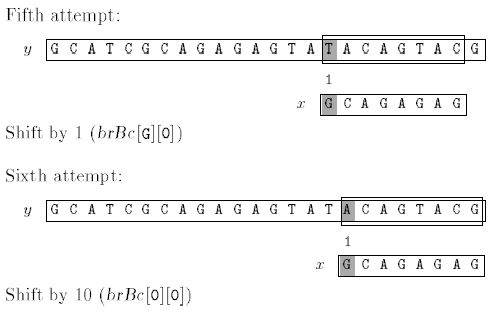
\includegraphics[width=0.9\textwidth]{img285.jpg}
	\caption{Lần 5--6: Kết thúc}
\end{figure}

\subsection{Lập trình theo thuật toán}

\begin{lstlisting}[style=CStyle]
void preBrBc(char *x, int m, int brBc[][ASIZE]) {
    int a, i;
    for (a = 0; a < ASIZE; ++a)
        for (i = 0; i < ASIZE; ++i)
            brBc[a][i] = m + 2;
    for (a = 0; a < ASIZE; ++a)
        brBc[a][(unsigned char)x[0]] = m + 1;
    for (i = 0; i < m - 1; ++i)
        brBc[(unsigned char)x[i]][(unsigned char)x[i+1]] = m-i;
    for (a = 0; a < ASIZE; ++a)
        brBc[(unsigned char)x[m-1]][a] = 1;
}

void BR(char *x, int m, char *y, int n) {
    int brBc[ASIZE][ASIZE], j;
    preBrBc(x, m, brBc);
    y[n] = y[n + 1] = '\0';
    j = 0;
    while (j <= n - m) {
        if (memcmp(x, y + j, m) == 0)
            OUTPUT(j);
        j += brBc[(unsigned char)y[j+m]]
                 [(unsigned char)y[j+m+1]];
    }
}
\end{lstlisting}

%-----------------------------------------------------------
\section{Thuật toán Apostolico-Giancarlo}
%-----------------------------------------------------------

\subsection{Trình bày thuật toán}

Thuật toán Apostolico-Giancarlo là biến thể của thuật toán Boyer-Moore. Thuật toán Boyer-Moore khó phân tích và sau mỗi lần thử nó quên hết tất cả các ký tự đã khớp trước đó. Apostolico-Giancarlo ghi nhớ độ dài của suffix dài nhất của mẫu $x$ sau mỗi lần thử. Thông tin này được lưu trong bảng \texttt{skip}. Giả sử trong 1 lần thử ở vị trí nhỏ hơn $j$, thuật toán đã match một suffix độ dài $k$ của $x$ ở vị trí $i + j$ $(0 < i < m)$ thì $\text{skip}[i+j] = k$. Nghĩa là $y[i+j-k+1..i+j] = x[m-1-k+1..m-1]$. Đặt $\text{suff}[i]$ $(0 \leq i < m)$ bằng độ dài suffix dài nhất của $x$ kết thúc ở vị trí $i$ trong $x$.

Trong lần thử tại vị trí $j$, nếu đoạn text $y[i+j+1..j+m-1]$ đã khớp với mẫu $x$ thì 4 trường hợp sau có thể xảy ra (với $k = \text{skip}[i+j]$ và $s = \text{suff}[i]$):

\begin{itemize}
	\item \textbf{TH 1}: $k > s$ và $s = i+1$. Điều đó có nghĩa rằng ta đã tìm thấy một mẫu $x$ trong $y$. Khi đó $\text{skip}[j+m-1] = m$.
	\item \textbf{TH 2}: $k > s$ và $s \leq i$. Điều đó có nghĩa là sự không khớp xảy ra giữa ký tự $x[i - \text{suff}[i]]$ và $y[i+j-\text{suff}[i]]$. Khi đó $\text{skip}[j+m-1] = m-1-i+\text{suff}[i]$. Bước dịch được thực hiện sử dụng $\text{bmBc}[y[i+j-\text{suff}[i]]]$ và $\text{bmGs}[i-\text{suff}[i]+1]$.
	\item \textbf{TH 3}: $k < s$, nghĩa là sự không khớp xảy ra giữa ký tự $x[i-k]$ và $y[i+j-k]$. Khi đó $\text{skip}[j+m-1] = m-1-i+k$. Bước dịch được thực hiện sử dụng $\text{bmBc}[y[i+j-k]]$ và $\text{bmGs}[i-k+1]$.
	\item \textbf{TH 4}: $k = s$. Đây là trường hợp duy nhất bước nhảy phải nhảy qua đoạn $y[i+j-k+1..i+j]$ để so sánh 2 ký tự $y[i+j-k]$ và $x[i-k]$.
\end{itemize}

Thuật toán Apostolico-Giancarlo sử dụng 2 cấu trúc dữ liệu:
\begin{itemize}
	\item Một bảng \texttt{skip} được cập nhật ở cuối mỗi lần thử $j$.
	\item Một bảng \texttt{suff} sử dụng để tính bảng \texttt{bmGs}.
\end{itemize}

\begin{figure}[H]
	\centering
	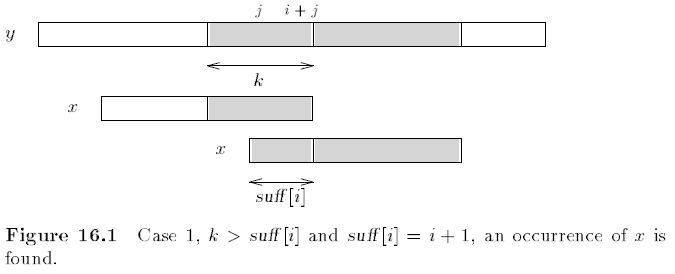
\includegraphics[width=0.7\textwidth]{img289.jpg}
	\caption{Trường hợp 1: $k > s$ và $s = i+1$}
\end{figure}
\begin{figure}[H]
	\centering
	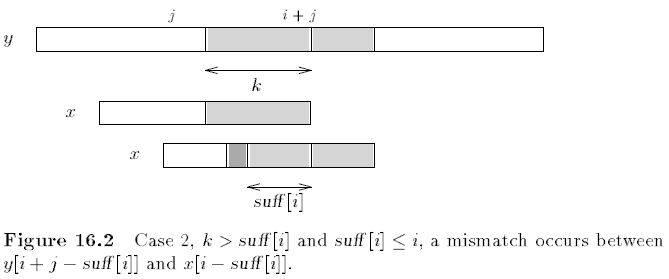
\includegraphics[width=0.7\textwidth]{img290.jpg}
	\caption{Trường hợp 2: $k > s$ và $s \leq i$}
\end{figure}
\begin{figure}[H]
	\centering
	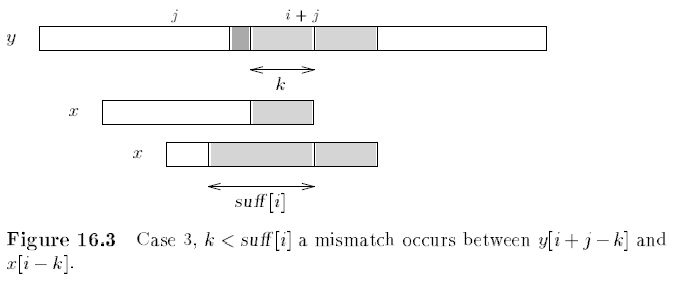
\includegraphics[width=0.7\textwidth]{img293.jpg}
	\caption{Trường hợp 3: $k < s$}
\end{figure}
\begin{figure}[H]
	\centering
	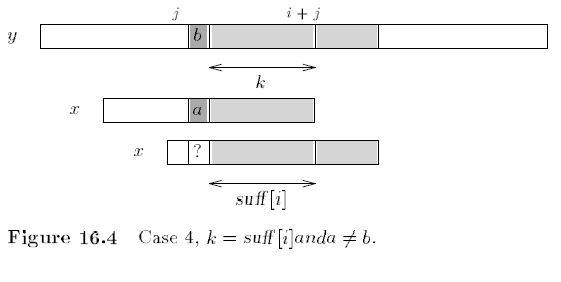
\includegraphics[width=0.7\textwidth]{img294.jpg}
	\caption{Trường hợp 4: $k = s$}
\end{figure}

\subsection{Đánh giá độ phức tạp thuật toán}

\begin{itemize}
	\item Pha xử lý: $O(m + \sigma)$.
	\item Pha tìm kiếm: $O(n)$, trường hợp xấu nhất $\frac{3}{2}n$ phép so sánh.
\end{itemize}

\subsection{Kiểm nghiệm thuật toán}

\begin{figure}[H]
	\centering
	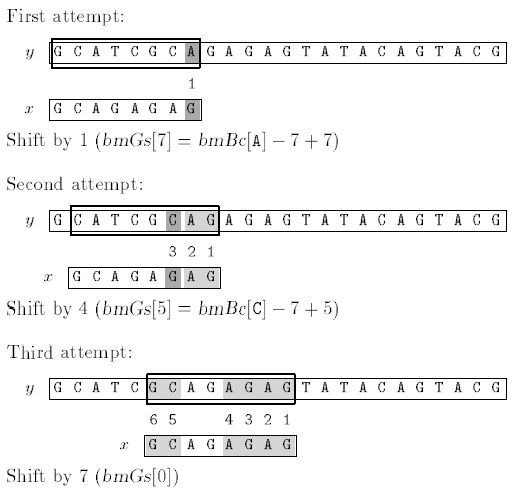
\includegraphics[width=0.9\textwidth]{img301.jpg}
	\caption{Lần 1--3: OUTPUT(5) ở lần 3}
\end{figure}
\begin{figure}[H]
	\centering
	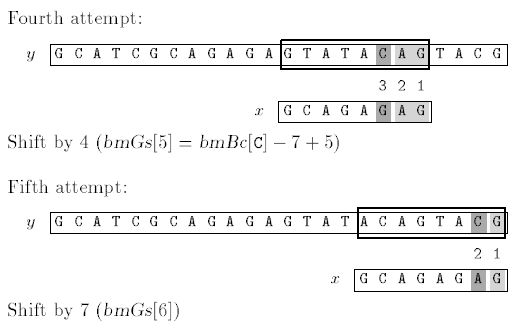
\includegraphics[width=0.9\textwidth]{img302.jpg}
	\caption{Lần 4--5: Kết thúc}
\end{figure}

\subsection{Lập trình theo thuật toán}

\begin{lstlisting}[style=CStyle]
void AG(char *x, int m, char *y, int n) {
    int bcShift, i, j, k, shift, s;
    int bmGs[XSIZE], bmBc[ASIZE], suff[XSIZE], skip[YSIZE];
    preBmGs(x, m, bmGs);
    preBmBc(x, m, bmBc);
    suffixes(x, m, suff);
    memset(skip, 0, n * sizeof(int));
    j = 0;
    while (j <= n - m) {
        i = m - 1;
        while (i >= 0) {
            k = skip[i + j];
            s = suff[i];
            if (k > 0) {
                if (k > s) { i -= s; break; }
                else if (k < s) { i -= k; break; }
                else i -= s;
            } else {
                if (x[i] == y[i + j]) --i;
                else break;
            }
        }
        if (i < 0) {
            OUTPUT(j);
            skip[j + m - 1] = m;
            shift = bmGs[0];
        } else {
            skip[i + j] = m - 1 - i;
            bcShift = bmBc[(unsigned char)y[i+j]] - m + 1 + i;
            shift = MAX(bmGs[i], bcShift);
        }
        j += shift;
    }
}
\end{lstlisting}

%=============================================================
\chapter{Tìm kiếm mẫu từ vị trí xác định}
%=============================================================

\section{Thuật toán Colussi}

\subsection{Trình bày thuật toán}

Thuật toán Colussi là sự cải tiến của thuật toán Knuth-Morris-Pratt. Các vị trí của mẫu (pattern) được chia làm 2 tập con. Các vị trí trong tập con thứ nhất được duyệt từ trái sang phải và các vị trí trong tập con thứ 2 (các vị trí còn lại) được duyệt từ phải sang trái. Mỗi lần thử (mỗi cửa sổ của văn bản $y$) gồm 2 pha (pha 1 luôn có, pha hai có thể có hoặc không):
\begin{itemize}
	\item \textbf{Pha 1} thực hiện so sánh từ trái sang phải các ký tự trong text với các ký tự trong pattern mà \texttt{kmpNext} có giá trị $> -1$. Những vị trí này trong pattern được gọi là \textbf{noholes}.
	\item \textbf{Pha 2} sẽ được thực hiện khi tất cả các so sánh trong pha 1 đều match. Nếu có 1 sự không khớp xảy ra trong pha 1 thuật toán sẽ dịch chuyển cửa sổ mà không thực hiện pha 2. Pha 2 so sánh các vị trí còn lại của pattern (các vị trí này gọi là \textbf{holes}) từ phải sang trái. Nếu có 1 sự không khớp xảy ra, thuật toán sẽ dịch chuyển cửa sổ sang vị trí tiếp theo.
\end{itemize}

Chiến lược này có 2 ưu điểm:
\begin{itemize}
	\item Khi 1 sự không khớp xảy ra trong pha 1, sau khi dịch chuyển cửa sổ thích hợp ta không cần phải so sánh các vị trí noholes đã so sánh trong cửa sổ trước.
	\item Khi 1 sự không khớp (mismatch) xảy ra trong pha 2, nghĩa là có 1 đoạn suffix của pattern đã match với 1 đoạn của text. Sau khi dịch chuyển cửa sổ thích hợp, 1 prefix của pattern sẽ match với 1 suffix của pattern, mà suffix này lại match với 1 đoạn của text $\Rightarrow$ prefix cũng sẽ match với đoạn text đó $\Rightarrow$ khi dịch chuyển cửa sổ, ta không cần phải so sánh đoạn text đó nữa.
\end{itemize}

\subsection{Đánh giá độ phức tạp thuật toán}

\begin{itemize}
	\item Pha tiền xử lý: $O(m)$.
	\item Pha tìm kiếm: $O(n)$.
\end{itemize}

\subsection{Kiểm nghiệm thuật toán}

\begin{figure}[H]
	\centering
	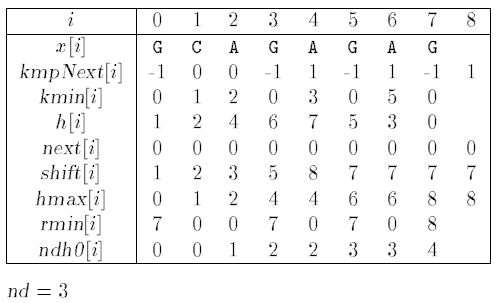
\includegraphics[width=0.9\textwidth]{img313.jpg}
	\caption{Bảng tiền xử lý Colussi cho $x = \texttt{GCAGAGAG}$}
\end{figure}
\begin{figure}[H]
	\centering
	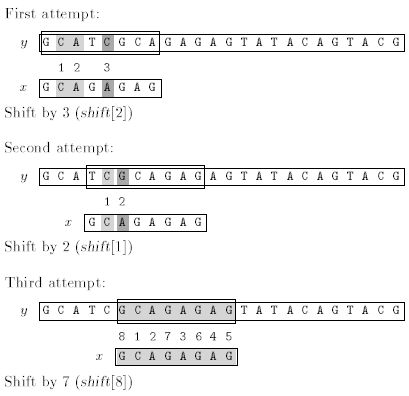
\includegraphics[width=0.9\textwidth]{img314.jpg}
	\caption{Lần 1--3: OUTPUT(5) ở lần 3}
\end{figure}
\begin{figure}[H]
	\centering
	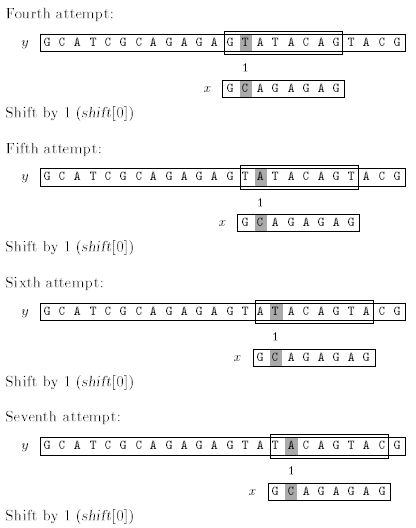
\includegraphics[width=0.9\textwidth]{img317.jpg}
	\caption{Lần 4--7}
\end{figure}
\begin{figure}[H]
	\centering
	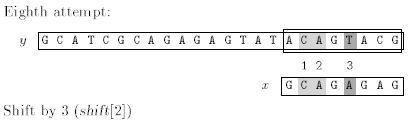
\includegraphics[width=0.9\textwidth]{img318.jpg}
	\caption{Lần 8: Kết thúc}
\end{figure}

\subsection{Lập trình theo thuật toán}

\begin{lstlisting}[style=CStyle]
int preColussi(char *x, int m, int h[], int next[], int shift[]) {
    int i, k, q, r, s, nd, kmin[XSIZE], rmin[XSIZE],
        hmax[XSIZE], nhd0[XSIZE], kmpNext[XSIZE];
    preKmp(x, m, kmpNext);
    for (i = 0; i <= m; ++i) hmax[i] = 0;
    for (k = 1; k < m; k += (k == kmpNext[k]+1) ? 1 : m) {
        q = 0;
        while (q + k <= m) { hmax[q] = q + k; q += k; }
    }
    for (i = 0; i < m; ++i) kmin[i] = rmin[i] = m;
    s = r = 0;
    for (i = 0; i < m; ++i) {
        if (hmax[i] == i + kmpNext[i + 1] + 1)
            h[s++] = i;
        else
            h[m - 1 - r++] = i;
    }
    nd = s;
    for (i = 0; i <= m; ++i) shift[i] = rmin[0];
    for (i = nd - 1; i >= 0; --i)
        shift[i] = kmin[h[i]];
    nhd0[0] = 0;
    for (i = 0; i < nd; ++i)
        nhd0[i+1] = nhd0[i] + (h[i] == 0 ? 0 : 1);
    for (i = 0; i <= nd; ++i) next[i] = nhd0[shift[i]];
    return nd;
}

void COLUSSI(char *x, int m, char *y, int n) {
    int i, j, last, nd, h[XSIZE], next[XSIZE], shift[XSIZE];
    nd = preColussi(x, m, h, next, shift);
    j = last = i = 0;
    while (j <= n - m) {
        while (i < m &&
               (last < j + h[i] || x[h[i]] == y[j + h[i]]))
            ++i;
        if (i >= m) {
            OUTPUT(j);
            last = j + m - 1;
        }
        j += shift[i];
        i = next[i];
    }
}
\end{lstlisting}

%-----------------------------------------------------------
\section{Thuật toán Skip Search}
%-----------------------------------------------------------

\subsection{Trình bày thuật toán}

Đối với mỗi ký tự trong bảng chữ cái, thuật toán Skip Search sử dụng một thùng (bucket) để chứa tất cả các vị trí của ký tự đó trong mẫu $x$. Khi một ký tự xuất hiện $k$ lần trong mẫu $x$, sẽ có $k$ vị trí tương ứng trong bucket của ký tự đó. Khi xâu $y$ chứa ít ký tự hơn so với bảng chữ cái, sẽ có một số bucket rỗng.

Pha tiền xử lý của thuật toán Skip Search sẽ tính bucket cho tất cả các ký tự trong bảng chữ cái. Đối với mỗi ký tự $c$ thuộc bảng chữ cái, ta có:
\[z[c] = \{i : 0 \leq i \leq m-1 \text{ và } x[i] = c\}\]
$z[c]$ chính là bucket của ký tự $c$.

Vòng lặp chính của pha tìm kiếm sẽ kiểm tra mỗi ký tự thứ $m$, $y[j]$ (do đó sẽ có $n/m$ lần lặp). Đối với mỗi $y[j]$, nó sẽ dùng mỗi vị trí trong bucket $z[y[j]]$ để kiểm tra xem liệu tại mỗi vị trí trong $z[y[j]]$ thì có tìm được một $x$ trong $y$ không. Nó thực hiện so sánh $x$ với $y$ từ vị trí đầu tiên, lần lượt tăng ký tự một cho đến khi gặp một sự không khớp hoặc tất cả đều khớp.

\subsection{Đánh giá độ phức tạp thuật toán}

\begin{itemize}
	\item Pha tiền xử lý: $O(m + \sigma)$.
	\item Pha tìm kiếm: $O(m \times n)$.
\end{itemize}

\subsection{Kiểm nghiệm thuật toán}

Bảng $z[c]$ cho $x = \texttt{GCAGAGAG}$:

\begin{center}
\begin{tabular}{|c|l|}
\hline
$c$ & $z[c]$ \\
\hline
A & $\{6, 4, 2\}$ \\
C & $\{1\}$ \\
G & $\{7, 5, 3, 0\}$ \\
T & $\emptyset$ \\
\hline
\end{tabular}
\end{center}

\begin{figure}[H]
	\centering
	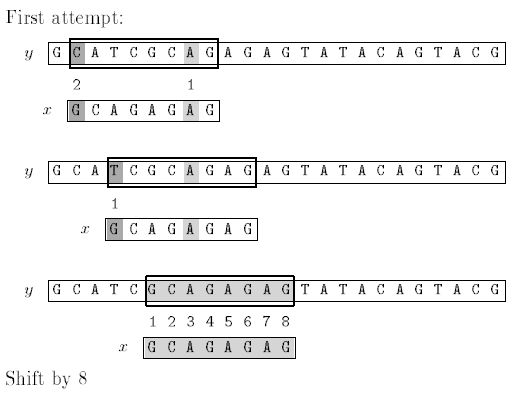
\includegraphics[width=0.9\textwidth]{img331.jpg}
	\caption{Pha tìm kiếm: OUTPUT(5)}
\end{figure}
\begin{figure}[H]
	\centering
	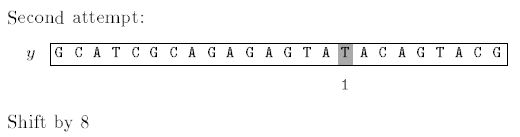
\includegraphics[width=0.9\textwidth]{img334.jpg}
	\caption{Tiếp tục tìm kiếm}
\end{figure}

\subsection{Lập trình theo thuật toán}

\begin{lstlisting}[style=CStyle]
void SKIP(char *x, int m, char *y, int n) {
    struct cell { int element; struct cell *next; };
    struct cell *z[ASIZE], *p;
    int i, j;
    for (i = 0; i < ASIZE; ++i) z[i] = NULL;
    for (i = m - 1; i >= 0; --i) {
        p = (struct cell *)malloc(sizeof(struct cell));
        p->element = i;
        p->next = z[(unsigned char)x[i]];
        z[(unsigned char)x[i]] = p;
    }
    for (j = m - 1; j < n; j += m) {
        p = z[(unsigned char)y[j]];
        while (p != NULL) {
            i = p->element;
            if (j - i + m - 1 > n - 1) break;
            if (j - i >= 0 && memcmp(x, y + j - i, m) == 0)
                OUTPUT(j - i);
            p = p->next;
        }
    }
}
\end{lstlisting}

%-----------------------------------------------------------
\section{Thuật toán Alpha Skip Search}
%-----------------------------------------------------------

\subsection{Trình bày thuật toán}

Là phiên bản cải tiến của thuật toán Skip Search, sử dụng các bucket để chứa các vị trí của mỗi factor độ dài $\log_\sigma m$.

Pha tiền xử lý của thuật toán Alpha Skip Search xây dựng một cây $T(x)$. Trong đó các nhánh của cây biểu diễn cho các factor độ dài $L = \log_\sigma m$ xuất hiện trong $x$. Sau đó, có một bucket tại mỗi lá của $T(x)$ để chứa các vị trí xuất hiện của factor (tương ứng với nhánh) trong $x$.

Pha tìm kiếm xem xét bucket của factor $y[j..j+L-1]$ với tất cả $j = k \times (m - L + 1) - 1$, với $k$ nằm trong đoạn $[1, \lfloor n/(m-L+1) \rfloor]$.

\subsection{Đánh giá độ phức tạp thuật toán}

\begin{itemize}
	\item Pha tiền xử lý: $O(m)$.
	\item Pha tìm kiếm: $O(m \times n)$.
\end{itemize}

\subsection{Kiểm nghiệm thuật toán}

Bảng $z[u]$ cho $x = \texttt{GCAGAGAG}$ với $q = 3$:

\begin{center}
\begin{tabular}{|c|c|}
\hline
$u$ (3-gram) & $z[u]$ \\
\hline
AGA & $\{4, 2\}$ \\
CAG & $\{1\}$ \\
GAG & $\{5, 3\}$ \\
GCA & $\{0\}$ \\
\hline
\end{tabular}
\end{center}

\begin{figure}[H]
	\centering
	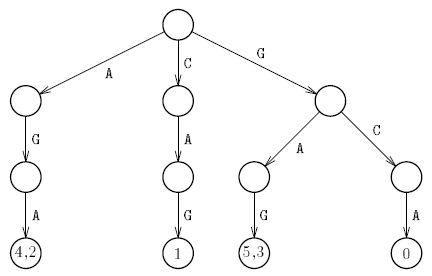
\includegraphics[width=0.9\textwidth]{img339.jpg}
	\caption{Trie của Alpha Skip với $q = 3$}
\end{figure}
\begin{figure}[H]
	\centering
	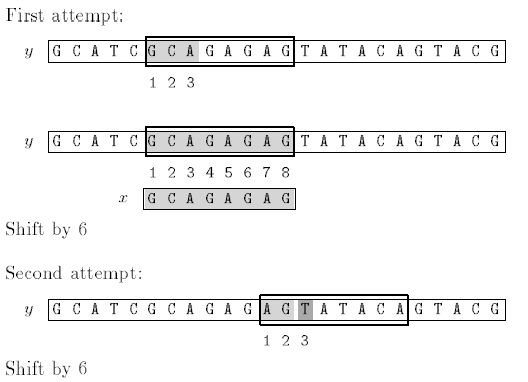
\includegraphics[width=0.9\textwidth]{img341.jpg}
	\caption{Lần 1: OUTPUT(5); Lần 2}
\end{figure}
\begin{figure}[H]
	\centering
	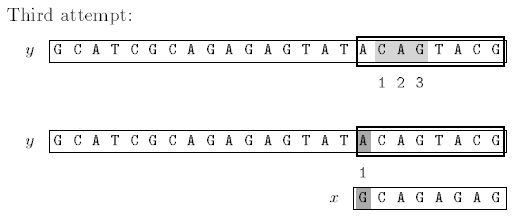
\includegraphics[width=0.9\textwidth]{img344.jpg}
	\caption{Lần 3: Kết thúc}
\end{figure}

\subsection{Lập trình theo thuật toán}

\begin{lstlisting}[style=CStyle]
void ALPHASKIP(char *x, int m, char *y, int n) {
    int logM, shift, b, j, q;
    for (logM = 1, q = ASIZE; q < m; q *= ASIZE, ++logM);
    /* Build trie and z lists */
    shift = m - logM + 1;
    for (j = m - logM; j < n - logM + 1; j += shift) {
        /* Traverse trie on y[j..j+logM-1]          */
        /* For each match in z[node]:                */
        /*   b = j - position_in_x                  */
        /*   if b >= 0 && b <= n-m                  */
        /*     if memcmp(x, y+b, m) == 0            */
        /*       OUTPUT(b)                           */
    }
}
\end{lstlisting}

%=============================================================
\chapter{Tìm kiếm mẫu từ vị trí bất kỳ}
%=============================================================

\section{Thuật toán Horspool}

\subsection{Trình bày thuật toán}

Thuật toán Horspool là phiên bản đơn giản hóa của thuật toán Boyer-Moore. Quy tắc dịch bad-character sử dụng trong thuật toán Boyer-Moore không hiệu quả đối với bảng chữ cái nhỏ, nhưng khi bảng chữ cái lớn so với độ dài của mẫu, như trường hợp với bảng ASCII và tìm kiếm thông thường trong một text editor thì nó trở nên rất hữu ích. Horspool đề xuất chỉ sử dụng bad-character shift của ký tự ngoài cùng bên phải cửa sổ (ký tự $y[j+m-1]$) để tính độ dịch.

\subsection{Đánh giá độ phức tạp thuật toán}

\begin{itemize}
	\item Pha tiền xử lý: độ phức tạp thời gian là $O(m + \sigma)$ và độ phức tạp bộ nhớ là $O(\sigma)$.
	\item Pha tìm kiếm có độ phức tạp thời gian là $O(m \times n)$.
\end{itemize}

\subsection{Kiểm nghiệm thuật toán}

\begin{figure}[H]
	\centering
	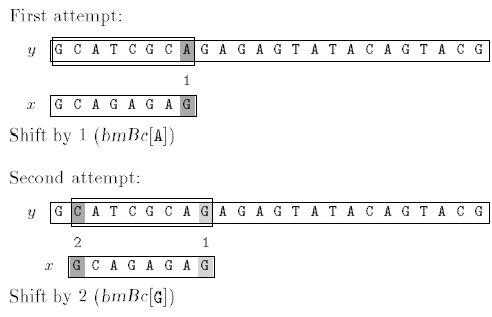
\includegraphics[width=0.9\textwidth]{img357.jpg}
	\caption{Lần 1--2}
\end{figure}
\begin{figure}[H]
	\centering
	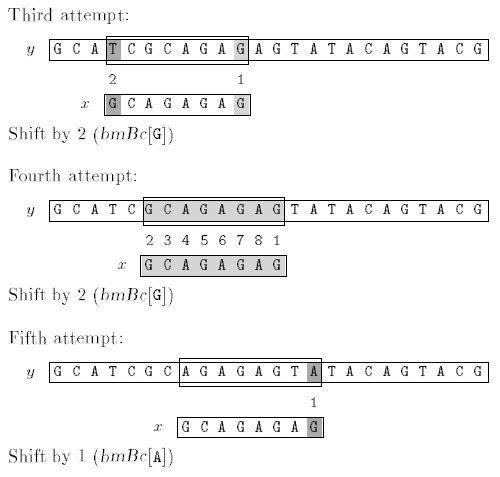
\includegraphics[width=0.9\textwidth]{img358.jpg}
	\caption{Lần 3--5: Lần 4 OUTPUT(5)}
\end{figure}
\begin{figure}[H]
	\centering
	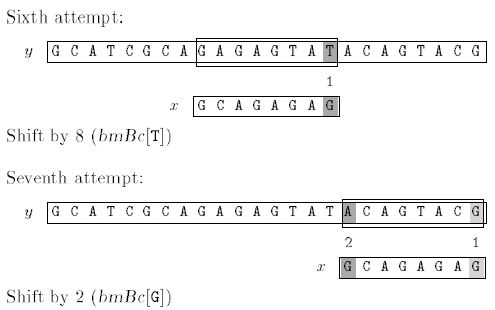
\includegraphics[width=0.9\textwidth]{img359.jpg}
	\caption{Lần 6--7: Kết thúc}
\end{figure}

\subsection{Lập trình theo thuật toán}

\begin{lstlisting}[style=CStyle]
void HORSPOOL(char *x, int m, char *y, int n) {
    int j, bmBc[ASIZE];
    char c;
    preBmBc(x, m, bmBc);
    j = 0;
    while (j <= n - m) {
        c = y[j + m - 1];
        if (x[m - 1] == c &&
            memcmp(x, y + j, m - 1) == 0)
            OUTPUT(j);
        j += bmBc[(unsigned char)c];
    }
}
\end{lstlisting}

%-----------------------------------------------------------
\section{Thuật toán Smith}
%-----------------------------------------------------------

\subsection{Trình bày thuật toán}

Thuật toán Smith sẽ giữ lại giá trị lớn nhất trong hai giá trị Horspool bad-character shift và Quick Search bad-character shift. Smith nhận thấy rằng độ dịch của ký tự ngay sau ký tự ngoài cùng bên phải ($y[j+m]$) đôi khi ngắn hơn độ dịch của ký tự ngoài cùng bên phải của cửa sổ ($y[j+m-1]$). Do đó, ông khuyên giữ lại giá trị lớn nhất trong 2 giá trị này. Pha tiền xử lý của thuật toán Smith sẽ tính các giá trị Horspool bad-character shift và Quick Search bad-character shift.

\subsection{Đánh giá độ phức tạp thuật toán}

\begin{itemize}
	\item Pha tiền xử lý: độ phức tạp thời gian là $O(m + \sigma)$ và độ phức tạp bộ nhớ là $O(\sigma)$.
	\item Pha tìm kiếm có độ phức tạp thời gian là $O(m \times n)$.
\end{itemize}

\subsection{Kiểm nghiệm thuật toán}

\begin{figure}[H]
	\centering
	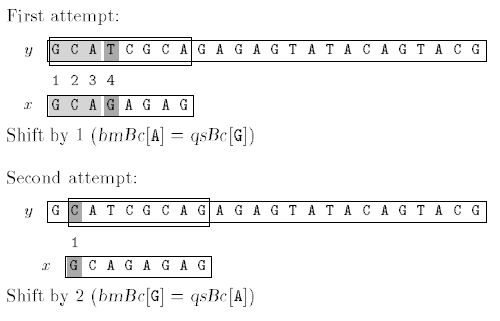
\includegraphics[width=0.9\textwidth]{img366.jpg}
	\caption{Lần 1--2}
\end{figure}
\begin{figure}[H]
	\centering
	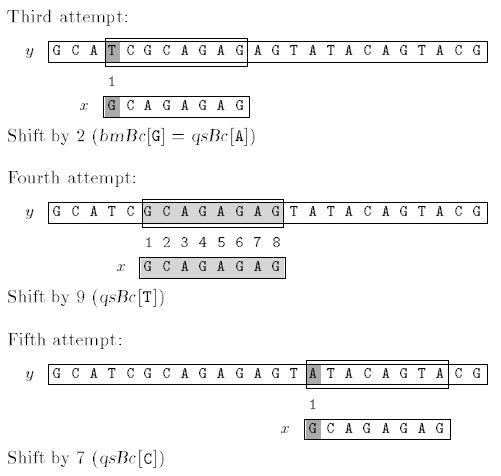
\includegraphics[width=0.9\textwidth]{img367.jpg}
	\caption{Lần 3--5: Lần 4 OUTPUT(5)}
\end{figure}

\subsection{Lập trình theo thuật toán}

\begin{lstlisting}[style=CStyle]
void SMITH(char *x, int m, char *y, int n) {
    int j, bmBc[ASIZE], qsBc[ASIZE];
    preBmBc(x, m, bmBc);
    preQsBc(x, m, qsBc);
    j = 0;
    while (j <= n - m) {
        if (memcmp(x, y + j, m) == 0)
            OUTPUT(j);
        j += MAX(bmBc[(unsigned char)y[j + m - 1]],
                 qsBc[(unsigned char)y[j + m]]);
    }
}
\end{lstlisting}

%-----------------------------------------------------------
\section{Thuật toán Raita}
%-----------------------------------------------------------

\subsection{Trình bày thuật toán}

Trong mỗi lần thử, đầu tiên thuật toán so sánh ký tự cuối của mẫu và ký tự cuối của cửa sổ, nếu khớp nó so sánh ký tự đầu tiên của mẫu và ký tự đầu tiên của cửa sổ, nếu khớp nó so sánh ký tự giữa của mẫu và của cửa sổ. Nếu vẫn khớp nó mới so sánh các ký tự còn lại, bắt đầu từ ký tự thứ 2. Bước dịch được tính như thuật toán Horspool.

\subsection{Đánh giá độ phức tạp thuật toán}

\begin{itemize}
	\item Pha tiền xử lý: độ phức tạp thời gian là $O(m + \sigma)$ và độ phức tạp bộ nhớ là $O(\sigma)$.
	\item Pha tìm kiếm có độ phức tạp thời gian là $O(m \times n)$.
\end{itemize}

\subsection{Kiểm nghiệm thuật toán}

\begin{figure}[H]
	\centering
	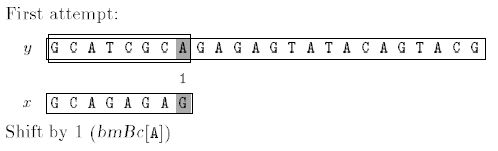
\includegraphics[width=0.9\textwidth]{img372.jpg}
	\caption{Lần 1: Kiểm tra ký tự cuối -- mismatch, dịch 1}
\end{figure}
\begin{figure}[H]
	\centering
	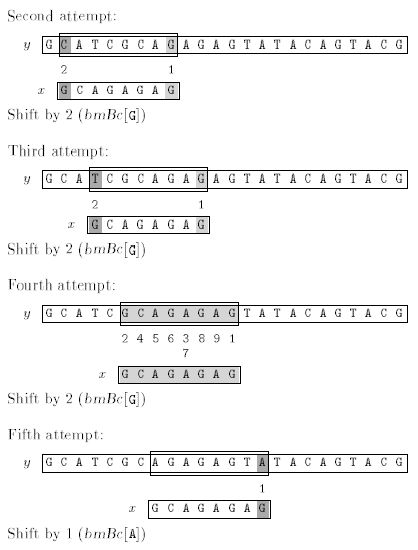
\includegraphics[width=0.9\textwidth]{img375.jpg}
	\caption{Lần 2--5: Lần 4 OUTPUT(5)}
\end{figure}
\begin{figure}[H]
	\centering
	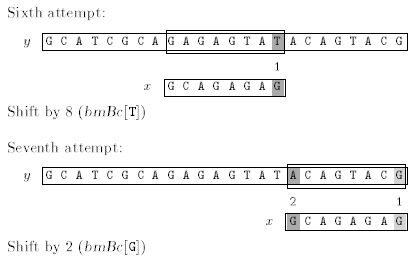
\includegraphics[width=0.9\textwidth]{img376.jpg}
	\caption{Lần 6--7: Kết thúc}
\end{figure}

\subsection{Lập trình theo thuật toán}

\begin{lstlisting}[style=CStyle]
void RAITA(char *x, int m, char *y, int n) {
    char firstCh, lastCh, middleCh;
    int j, bmBc[ASIZE];
    preBmBc(x, m, bmBc);
    firstCh  = x[0];
    middleCh = x[m / 2];
    lastCh   = x[m - 1];
    j = 0;
    while (j <= n - m) {
        if (lastCh   == y[j + m - 1] &&
            middleCh == y[j + m / 2] &&
            firstCh  == y[j] &&
            memcmp(x + 1, y + j + 1, m - 2) == 0)
            OUTPUT(j);
        j += bmBc[(unsigned char)y[j + m - 1]];
    }
}
\end{lstlisting}

\end{document}
